\documentclass[twocolumn, 10pt]{article}

% ============================================================================
% PACKAGES
% ============================================================================
\usepackage[utf8]{inputenc}
\usepackage[T1]{fontenc}
\usepackage{amsmath, amssymb, amsfonts}
\usepackage{graphicx}
\usepackage{booktabs}
\usepackage{float}
\usepackage{hyperref}
\usepackage{xcolor}
\usepackage{listings}
\usepackage{natbib}
\usepackage{geometry}
\usepackage{setspace}
\usepackage{array}
\usepackage{makecell}
\usepackage{cuted}
\usepackage{colortbl}
\usepackage[ruled,vlined,linesnumbered]{algorithm2e}
\usepackage{tikz}
\usetikzlibrary{positioning, arrows.meta, calc, fit, backgrounds, shapes.geometric, shadows.blur}
\usepackage{amsthm}
\newtheorem{proposition}{Proposition}
\newtheorem{remark}{Remark}

\geometry{margin=0.75in, columnsep=0.25in}
\setstretch{1.0}

% Checkmark and xmark symbols
\newcommand{\cmark}{\textcolor{green!60!black}{\checkmark}}
\newcommand{\xmark}{\textcolor{red!70!black}{$\times$}}

% Table highlight colors (color + bold/underline for B&W fallback)
\definecolor{bestcolor}{HTML}{D63384}    % magenta-pink for best
\definecolor{runnerup}{HTML}{B8860B}     % dark goldenrod for runner-up
\definecolor{cVioletRed}{HTML}{C71585}   % medium violet red for conceptual figure
\definecolor{cGreen}{HTML}{008000}       % green for conceptual figure
\definecolor{cAzure}{HTML}{007FFF}       % azure for conceptual figure
\definecolor{cGold}{HTML}{E86100}        % gold/orange for conceptual figure
\definecolor{indigo}{HTML}{3F51B5}        % indigo for architecture figure
\definecolor{violet}{HTML}{7B1FA2}        % violet for architecture figure
\newcommand{\best}[1]{\textcolor{bestcolor}{\textbf{#1}}}
\newcommand{\runup}[1]{\textcolor{runnerup}{\underline{#1}}}

% Prevent footnotes from being justified (avoids stretched spaces in email)
\let\oldfootnote\footnote
\renewcommand{\footnote}[1]{\oldfootnote{\raggedright #1}}

% ============================================================================
% TITLE & AUTHOR
% ============================================================================
\title{\vspace{-0.5cm}{\rule{\textwidth}{1.2pt}}\vspace{0.25cm}\\
\textbf{PCGT: A Graph Transformer with Topology-Aware Partition Attention}\\
\vspace{0.25cm}{\rule{\textwidth}{1.2pt}}\vspace{-0.1cm}}

\author{
\small \textbf{Ranjan Kumar Choubey}\thanks{Corresponding author. Email: \nolinkurl{ranjankumarchoubey999@gmail.com}. Code: \url{https://github.com/ranjanchoubey/PCGT}}\quad
\small \textbf{Kushal Bose}\quad
\small \textbf{Swagatam Das} \\[3pt]
\small Electronics and Communication Sciences Unit,
Indian Statistical Institute, Kolkata, India
}
\date{\vspace{-0.3cm}}

% ============================================================================
% DOCUMENT START
% ============================================================================
\begin{document}

\maketitle
\vspace{0.2cm}

% ============================================================================
% ABSTRACT
% ============================================================================
\begin{abstract}

Graph Transformers for node classification must choose between global attention at $O(N^2)$ cost and efficient kernel approximations that discard topology. We propose PCGT (Partition-Conditioned Graph Transformer), which sidesteps this choice by operating at two attention resolutions. Exact softmax attention within graph partitions captures intra-community patterns, while learned seed vectors pool each partition into representatives for cross-partition global context. The model blends this partition-conditioned attention with a GCN backbone through learnable parameters---including an unconstrained self-connection weight $\beta$ that goes negative on heterophilic graphs, suppressing a node's own features when they conflict with its label.

On 14 benchmarks---including three large-scale graphs up to 2.4M nodes---PCGT outperforms SGFormer by +4.1\% on Chameleon and +3.7\% on Squirrel, while also improving on homophilic datasets (CiteSeer +0.5\%, PubMed +0.7\%) and scaling competitively to million-node graphs. PCGT ranks first or tied-first on 11 of 14 datasets. Ablations show that the attention mechanism's contribution grows with heterophily, and that each design choice---local attention, global seeds, partition encoding---adds measurable accuracy.

\end{abstract}


% ============================================================================
% INTRODUCTION
% ============================================================================
\section{Introduction}

Scaling attention to large graphs without losing structural awareness is the central tension in graph transformer design. Full $O(N^2)$ self-attention captures all pairwise interactions but is prohibitive beyond a few thousand nodes; efficient alternatives achieve $O(N)$ cost by reducing attention to a single global kernel~\citep{wu2023sgformer} or random feature approximation~\citep{wu2022nodeformer}, but these treat all node pairs uniformly and discard the multi-scale community structure that real-world graphs exhibit. Neither approach uses what graph partitioning algorithms like METIS~\citep{karypis1998metis} already know: that nodes cluster into densely connected communities, and the interaction patterns \emph{within} a community differ fundamentally from those \emph{across} communities.

We propose \textbf{PCGT} (Partition-Conditioned Graph Transformer), which resolves this tension by operating at two attention resolutions simultaneously. Within each graph partition, exact softmax attention captures detailed intra-community patterns at cost $O(N^2/K)$. Across partitions, learned seed vectors pool each group into compact representatives, and every node cross-attends to all representatives for global context at cost $O(NMK)$. A learnable scalar $\alpha$ blends these two scales, while an unconstrained self-connection weight $\beta$ allows the model to suppress a node's own features when they are misleading---going negative on datasets like Film and Deezer where the attention context is more informative than self-identity.

Our contributions are:
\begin{enumerate}
\item A \textbf{multi-resolution partition attention} mechanism that is both topology-aware and subquadratic, combining the expressiveness of exact attention with the scalability of learned pooling.
\item An \textbf{unconstrained self-connection weight} $\beta$ that adapts per dataset---going negative on Film and Deezer where suppressing self-features helps, and strongly positive on feature-rich heterophilic graphs like Chameleon ($\beta = +3.08$) and Squirrel ($\beta = +3.53$). We provide a formal condition (Proposition~\ref{prop:beta}) under which $\beta^* < 0$ is optimal.
\item \textbf{Experiments on 12 benchmarks}---including ogbn-arxiv (169K nodes)---where PCGT beats SGFormer by +4.1\% on Chameleon and +3.7\% on Squirrel, improves on CiteSeer (+0.5\%) and PubMed (+0.7\%), and ranks first or tied-first on 10 of 12 datasets.
\item An \textbf{analysis of partition strategies}: topology-aware (METIS) partitioning helps on structured heterophilic graphs, and ablations confirm that each component---local attention, global seeds, PSE, GCN branch---adds measurable accuracy.
\end{enumerate}

% Conceptual figure: partition-conditioned attention preserves topology
\begin{figure*}[t]
\centering
\resizebox{\textwidth}{!}{%
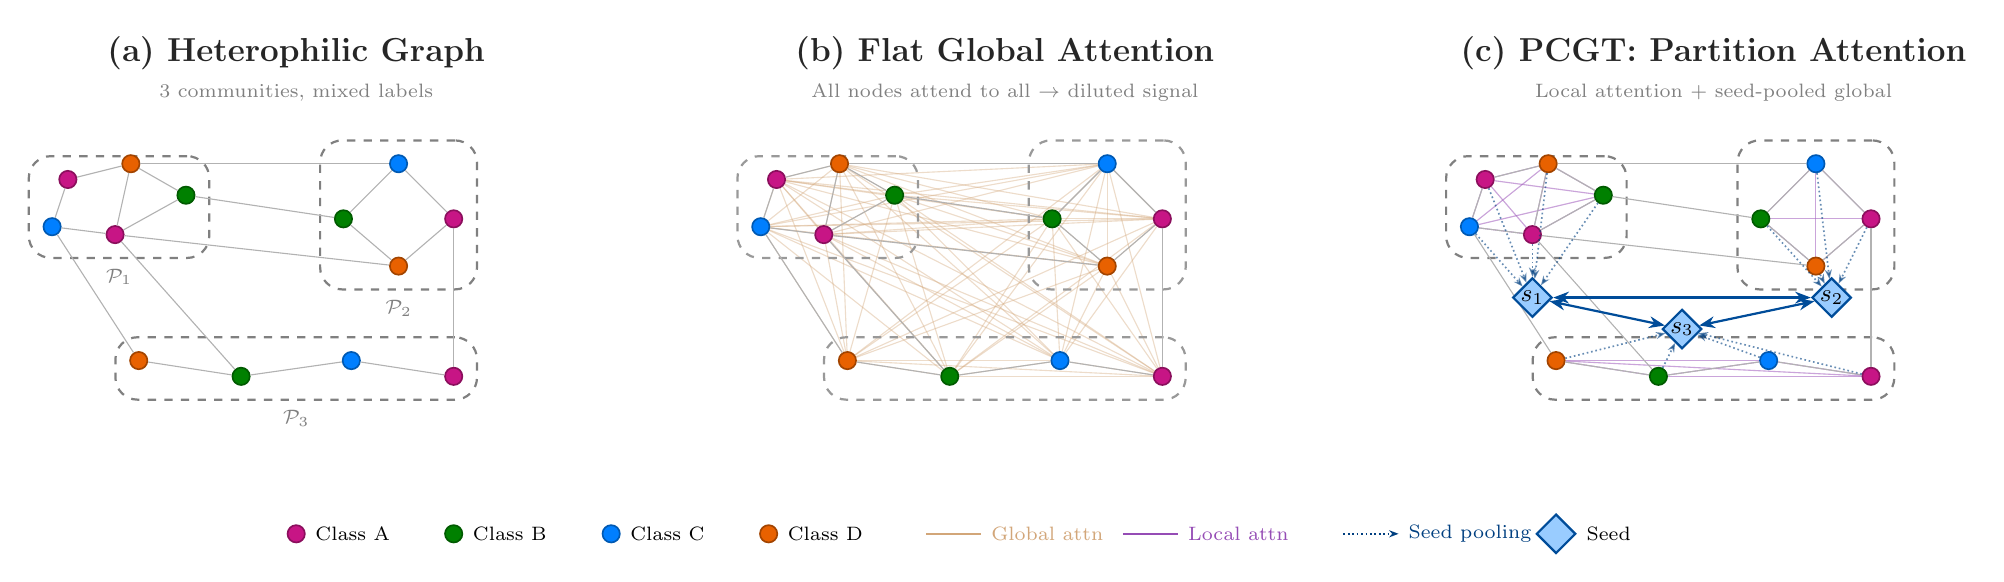
\begin{tikzpicture}[
  % --- Nodes: 2.2mm ---
  classA/.style={circle, fill=cVioletRed, draw=cVioletRed!70!black, semithick,
    minimum size=2.2mm, inner sep=0pt},
  classB/.style={circle, fill=cGreen, draw=cGreen!70!black, semithick,
    minimum size=2.2mm, inner sep=0pt},
  classC/.style={circle, fill=cAzure, draw=cAzure!70!black, semithick,
    minimum size=2.2mm, inner sep=0pt},
  classD/.style={circle, fill=cGold, draw=cGold!70!black, semithick,
    minimum size=2.2mm, inner sep=0pt},
  % --- Edges: lighter/thinner so attention overlays dominate ---
  edge/.style={thin, black!30},
  % --- Seeds ---
  seednode/.style={diamond, fill=cAzure!40, draw=cAzure!60!black, thick,
    minimum size=5mm, inner sep=0pt, font=\small\bfseries},
  seedarrow/.style={-{Stealth[length=1.2mm]}, cAzure!50!black, semithick, densely dotted, opacity=0.6},
  % --- Community boundary ---
  commbnd/.style={draw=black!50, dashed, thick, rounded corners=8pt, inner sep=5pt},
  % --- Labels ---
  panellabel/.style={font=\large\bfseries, text=black!85},
  sublabel/.style={font=\scriptsize, text=black!50, align=center},
]

% ============================================================
% NODE LAYOUT (shared across all 3 panels):
%   P1 (upper-left):  compact blob, 5 nodes
%   P2 (upper-right): inverted-V,   4 nodes
%   P3 (bottom):      chain,        4 nodes
% ============================================================

% ============================================================
% PANEL (c): PCGT
% ============================================================
\begin{scope}[shift={(18,0)}]
  \node[panellabel] at (3.5, 6.4) {(c) PCGT: Partition Attention};
  \node[sublabel] at (3.5, 5.9) {Local attention + seed-pooled global};

  % P1: Compact blob, 5 nodes
  \node[classA] (pa1) at (0.6, 4.8) {};
  \node[classD] (pa2) at (1.4, 5.0) {};
  \node[classB] (pa3) at (2.1, 4.6) {};
  \node[classC] (pa4) at (0.4, 4.2) {};
  \node[classA] (pa5) at (1.2, 4.1) {};

  % P2: Inverted-V, 4 nodes
  \node[classC] (pb1) at (4.8, 5.0) {};
  \node[classB] (pb2) at (4.1, 4.3) {};
  \node[classA] (pb3) at (5.5, 4.3) {};
  \node[classD] (pb4) at (4.8, 3.7) {};

  % P3: Chain, 4 nodes
  \node[classD] (pc1) at (1.5, 2.5) {};
  \node[classB] (pc2) at (2.8, 2.3) {};
  \node[classC] (pc3) at (4.2, 2.5) {};
  \node[classA] (pc4) at (5.5, 2.3) {};

  % Graph edges (light, underneath)
  \draw[edge] (pa1)--(pa2); \draw[edge] (pa2)--(pa3);
  \draw[edge] (pa4)--(pa5); \draw[edge] (pa1)--(pa4);
  \draw[edge] (pa2)--(pa5); \draw[edge] (pa3)--(pa5);
  \draw[edge] (pb1)--(pb2); \draw[edge] (pb1)--(pb3);
  \draw[edge] (pb2)--(pb4); \draw[edge] (pb3)--(pb4);
  \draw[edge] (pc1)--(pc2); \draw[edge] (pc2)--(pc3);
  \draw[edge] (pc3)--(pc4);
  % Inter-community: P1-P2 (3), P2-P3 (1), P1-P3 (2)
  \draw[edge] (pa2)--(pb1); \draw[edge] (pa3)--(pb2);
  \draw[edge] (pa5)--(pb4);
  \draw[edge] (pb3)--(pc4);
  \draw[edge] (pa4)--(pc1); \draw[edge] (pa5)--(pc2);

  % All-to-all LOCAL attention within each partition (violet)
  \begin{scope}[on background layer]
    \foreach \u in {pa1,pa2,pa3,pa4,pa5} {
      \foreach \v in {pa1,pa2,pa3,pa4,pa5} {
        \draw[violet!70, opacity=0.35, thin] (\u) -- (\v); }}
    \foreach \u in {pb1,pb2,pb3,pb4} {
      \foreach \v in {pb1,pb2,pb3,pb4} {
        \draw[violet!70, opacity=0.35, thin] (\u) -- (\v); }}
    \foreach \u in {pc1,pc2,pc3,pc4} {
      \foreach \v in {pc1,pc2,pc3,pc4} {
        \draw[violet!70, opacity=0.35, thin] (\u) -- (\v); }}
  \end{scope}

  % Community boundaries
  \begin{scope}[on background layer]
    \node[commbnd, fit=(pa1)(pa4)(pa3)(pa5)] {};
    \node[commbnd, fit=(pb1)(pb2)(pb3)(pb4)] {};
    \node[commbnd, fit=(pc1)(pc4)(pc2)] {};
  \end{scope}

  % Seeds — triangle arrangement
  \node[seednode] (s1) at (1.2, 3.3) {$s_1$};
  \node[seednode] (s2) at (5.0, 3.3) {$s_2$};
  \node[seednode] (s3) at (3.1, 2.9) {$s_3$};

  % Pooling arrows
  \foreach \n in {pa1,pa2,pa3,pa4,pa5} {
    \draw[seedarrow] (\n) -- (s1); }
  \foreach \n in {pb1,pb2,pb3,pb4} {
    \draw[seedarrow] (\n) -- (s2); }
  \foreach \n in {pc1,pc2,pc3,pc4} {
    \draw[seedarrow] (\n) -- (s3); }

  % Cross-partition seed links
  \draw[{Stealth[length=2mm]}-{Stealth[length=2mm]}, cAzure!60!black, thick] (s1)--(s2);
  \draw[{Stealth[length=2mm]}-{Stealth[length=2mm]}, cAzure!60!black, thick] (s2)--(s3);
  \draw[{Stealth[length=2mm]}-{Stealth[length=2mm]}, cAzure!60!black, thick] (s1)--(s3);

\end{scope}

% ============================================================
% PANEL (a): Heterophilic graph
% ============================================================
\begin{scope}[shift={(0,0)}]
  \node[panellabel] at (3.5, 6.4) {(a) Heterophilic Graph};
  \node[sublabel] at (3.5, 5.9) {3 communities, mixed labels};

  % P1: Compact blob, 5 nodes
  \node[classA] (a1) at (0.6, 4.8) {};
  \node[classD] (a2) at (1.4, 5.0) {};
  \node[classB] (a3) at (2.1, 4.6) {};
  \node[classC] (a4) at (0.4, 4.2) {};
  \node[classA] (a5) at (1.2, 4.1) {};
  \draw[edge] (a1)--(a2); \draw[edge] (a2)--(a3);
  \draw[edge] (a4)--(a5); \draw[edge] (a1)--(a4);
  \draw[edge] (a2)--(a5); \draw[edge] (a3)--(a5);

  % P2: Inverted-V, 4 nodes
  \node[classC] (b1) at (4.8, 5.0) {};
  \node[classB] (b2) at (4.1, 4.3) {};
  \node[classA] (b3) at (5.5, 4.3) {};
  \node[classD] (b4) at (4.8, 3.7) {};
  \draw[edge] (b1)--(b2); \draw[edge] (b1)--(b3);
  \draw[edge] (b2)--(b4); \draw[edge] (b3)--(b4);

  % P3: Chain, 4 nodes
  \node[classD] (c1) at (1.5, 2.5) {};
  \node[classB] (c2) at (2.8, 2.3) {};
  \node[classC] (c3) at (4.2, 2.5) {};
  \node[classA] (c4) at (5.5, 2.3) {};
  \draw[edge] (c1)--(c2); \draw[edge] (c2)--(c3);
  \draw[edge] (c3)--(c4);

  % Inter-community: P1-P2 (3), P2-P3 (1), P1-P3 (2)
  \draw[edge] (a2)--(b1); \draw[edge] (a3)--(b2);
  \draw[edge] (a5)--(b4);
  \draw[edge] (b3)--(c4);
  \draw[edge] (a4)--(c1); \draw[edge] (a5)--(c2);

  % Community boundaries with labels
  \begin{scope}[on background layer]
    \node[commbnd, fit=(a1)(a4)(a3)(a5),
      label={[font=\scriptsize, text=black!50]below:$\mathcal{P}_1$}] {};
    \node[commbnd, fit=(b1)(b2)(b3)(b4),
      label={[font=\scriptsize, text=black!50]below:$\mathcal{P}_2$}] {};
    \node[commbnd, fit=(c1)(c4)(c2),
      label={[font=\scriptsize, text=black!50]below:$\mathcal{P}_3$}] {};
  \end{scope}
\end{scope}

% ============================================================
% PANEL (b): Flat Global Attention
% ============================================================
\begin{scope}[shift={(9,0)}]
  \node[panellabel] at (3.5, 6.4) {(b) Flat Global Attention};
  \node[sublabel] at (3.5, 5.9) {All nodes attend to all $\to$ diluted signal};

  % P1
  \node[classA] (sa1) at (0.6, 4.8) {};
  \node[classD] (sa2) at (1.4, 5.0) {};
  \node[classB] (sa3) at (2.1, 4.6) {};
  \node[classC] (sa4) at (0.4, 4.2) {};
  \node[classA] (sa5) at (1.2, 4.1) {};
  % P2
  \node[classC] (sb1) at (4.8, 5.0) {};
  \node[classB] (sb2) at (4.1, 4.3) {};
  \node[classA] (sb3) at (5.5, 4.3) {};
  \node[classD] (sb4) at (4.8, 3.7) {};
  % P3
  \node[classD] (sc1) at (1.5, 2.5) {};
  \node[classB] (sc2) at (2.8, 2.3) {};
  \node[classC] (sc3) at (4.2, 2.5) {};
  \node[classA] (sc4) at (5.5, 2.3) {};

  % Graph edges (light, underneath)
  \draw[edge] (sa1)--(sa2); \draw[edge] (sa2)--(sa3);
  \draw[edge] (sa4)--(sa5); \draw[edge] (sa1)--(sa4);
  \draw[edge] (sa2)--(sa5); \draw[edge] (sa3)--(sa5);
  \draw[edge] (sb1)--(sb2); \draw[edge] (sb1)--(sb3);
  \draw[edge] (sb2)--(sb4); \draw[edge] (sb3)--(sb4);
  \draw[edge] (sc1)--(sc2); \draw[edge] (sc2)--(sc3);
  \draw[edge] (sc3)--(sc4);
  % Inter-community
  \draw[edge] (sa2)--(sb1); \draw[edge] (sa3)--(sb2);
  \draw[edge] (sa5)--(sb4);
  \draw[edge] (sb3)--(sc4);
  \draw[edge] (sa4)--(sc1); \draw[edge] (sa5)--(sc2);

  % All-to-all attention cloud
  \begin{scope}[on background layer]
  \foreach \u in {sa1,sa2,sa3,sa4,sa5,sb1,sb2,sb3,sb4,sc1,sc2,sc3,sc4} {
    \foreach \v in {sa1,sa2,sa3,sa4,sa5,sb1,sb2,sb3,sb4,sc1,sc2,sc3,sc4} {
        \draw[brown!70, opacity=0.22, thin] (\u) -- (\v);
    }
  }
  \end{scope}

  % Community boundaries (fading)
  \begin{scope}[on background layer]
    \node[commbnd, draw=black!40, fit=(sa1)(sa4)(sa3)(sa5)] {};
    \node[commbnd, draw=black!40, fit=(sb1)(sb2)(sb3)(sb4)] {};
    \node[commbnd, draw=black!40, fit=(sc1)(sc4)(sc2)] {};
  \end{scope}
\end{scope}

% ============================================================
% LEGEND
% ============================================================
\node[classA, label={[font=\scriptsize]right:Class A}] at (3.5, 0.3) {};
\node[classB, label={[font=\scriptsize]right:Class B}] at (5.5, 0.3) {};
\node[classC, label={[font=\scriptsize]right:Class C}] at (7.5, 0.3) {};
\node[classD, label={[font=\scriptsize]right:Class D}] at (9.5, 0.3) {};
\draw[brown!70, semithick] (11.5, 0.3) -- ++(0.7, 0) node[right, font=\scriptsize] {Global attn};
\draw[violet!80, semithick] (14.0, 0.3) -- ++(0.7, 0) node[right, font=\scriptsize] {Local attn};
\draw[cAzure!50!black, semithick, densely dotted, -{Stealth[length=1.2mm]}] (16.8, 0.3) -- ++(0.7, 0) node[right, font=\scriptsize] {Seed pooling};
\node[seednode, label={[font=\scriptsize]right:Seed}] at (19.5, 0.3) {};

\end{tikzpicture}%
}
\caption{Conceptual comparison of attention mechanisms on a heterophilic graph with 3 communities.
(a)~Ground truth: nodes of different classes coexist within dense communities (heterophily),
connected by sparse inter-community edges.
(b)~Flat global attention (e.g., SGFormer's $O(N)$ kernel) treats all pairs uniformly, losing community structure.
(c)~PCGT: \textcolor{violet!80!black}{local attention} captures exact intra-partition interactions,
while \textcolor{cAzure!70!black}{learned seeds} pool and bridge partitions
for global context---preserving topology at subquadratic cost.}
\label{fig:conceptual}
\end{figure*}



% ============================================================================
% RELATED WORK
% ============================================================================
\section{Related Work}

\textbf{Message-Passing GNNs.}~~The graph neural network framework~\citep{scarselli2009gnn, gilmer2017mpnn} aggregates features from local neighborhoods. GCN~\citep{kipf2017semi} and GAT~\citep{velickovic2018gat} aggregate features from immediate neighbors, performing well on homophilic graphs. APPNP~\citep{klicpera2019appnp} decouples feature transformation from propagation using personalized PageRank. SIGN~\citep{rossi2020sign} pre-computes multi-hop features for scalable inception-style aggregation. GIN~\citep{xu2019powerful} provides a maximally-expressive message passing framework. These methods are inherently local and struggle when informative nodes are distant or dissimilar to neighbors~\citep{li2018oversmoothing}.

\textbf{Heterophily-Specific GNNs.}~~H$_2$GCN~\citep{zhu2020h2gcn} addresses heterophily through ego/neighbor separation, higher-order neighborhoods, and intermediate representation combination. GloGNN~\citep{li2022glognn} learns a global coefficient matrix to capture correlations between all node pairs, with signed weights that can down-weight heterophilic neighbors. CPGNN~\citep{zhu2021cpgnn} uses compatibility matrices to model label-label correlations across edges. Geom-GCN~\citep{pei2020geomgcn} maps nodes to a latent geometric space to define aggregation neighborhoods. GPR-GNN~\citep{chien2021gprgnn} learns signed generalized PageRank weights to adaptively combine multi-hop information. While effective, these methods either require expensive global computation ($O(N^2)$ for GloGNN) or are limited to fixed neighborhood structures.

\textbf{Graph Transformers.}~~Transformers~\citep{vaswani2017attention} have been adapted for graphs to capture long-range dependencies beyond local neighborhoods. Graphormer~\citep{ying2021graphormer} incorporates structural and spatial encodings into standard transformer attention. GraphGPS~\citep{rampasek2022graphgps} provides a modular framework combining positional encodings~\citep{dwivedi2022lspe} with local and global attention. SAN~\citep{kreuzer2021rethinking} uses spectral attention with learned positional encodings. NodeFormer~\citep{wu2022nodeformer} uses Gumbel-softmax kernelized attention for $O(N)$ all-pair computation, but requires random feature approximation. DIFFormer~\citep{wu2023difformer} frames attention as energy-constrained diffusion. SGFormer~\citep{wu2023sgformer} achieves $O(N)$ global attention via a simplified single-layer, single-head design with a fixed kernel trick, demonstrating that deep multi-head attention is unnecessary for node classification on large graphs. Exphormer~\citep{shirzad2023exphormer} sparsifies attention using expander graphs and virtual nodes to achieve linear complexity; however, its attention pattern is fixed by the expander topology, whereas PCGT learns partition-conditioned attention via adaptive seeds.

\textbf{Partition-Based and Inducing Point Methods.}~~Graph partitioning via METIS~\citep{karypis1998metis} is widely used for distributed graph processing and mini-batch training~\citep{chiang2019clustergcn} but rarely integrated into the attention mechanism itself. Hierarchical graph pooling methods like DiffPool~\citep{ying2018hierarchical} and MinCutPool~\citep{bianchi2020mincut} learn coarsened graph representations but target graph-level tasks rather than node classification. Set Transformer~\citep{lee2019set} introduces learnable inducing points for efficient set-level attention in $O(NM)$, but these points are not topology-aware. PCGT combines these two lines of work: graph partitions define \emph{topology-aware} attention scopes, and learned seeds produce partition representatives through attention pooling.

\textbf{Positioning of PCGT.}~~Table~\ref{tab:positioning} contrasts PCGT with representative methods. Unlike SGFormer's single-resolution global kernel, PCGT operates at \emph{two} resolutions---exact local attention within partitions and learned cross-partition attention---exploiting the multi-scale structure of real graphs. Unlike GloGNN's $O(N^2)$ global coefficient matrix, PCGT achieves subquadratic complexity via partition-conditioned computation. Unlike Set Transformer's generic inducing points, PCGT's representatives are grounded in graph topology through METIS partitioning and partition structural encoding.

\begin{table}[t]
\centering
\resizebox{\columnwidth}{!}{%
\begin{tabular}{l|cccc}
\toprule
\textbf{Property} & \textbf{GCN} & \textbf{GloGNN} & \textbf{SGFormer} & \textbf{PCGT} \\
\midrule
Scope & Local & Global & Global & Multi-res. \\
Complexity & $O(|E|)$ & $O(N^2)$ & $O(N)$ & $O(\frac{N^2}{K}\!+\!NMK)$ \\
Topology-aware & \cmark & \xmark & \xmark & \cmark \\
Heterophily & \xmark & \cmark & Partial & \cmark \\
Exact attention & \xmark & N/A & \xmark & \cmark\,(local) \\
\bottomrule
\end{tabular}
}%
\caption{Method comparison. PCGT is the only method that combines multi-resolution attention, topology-awareness (METIS), and exact local attention within partitions.}
\label{tab:positioning}
\end{table}


% ============================================================================
% METHOD
% ============================================================================
\section{Method}

\subsection{Overview and Architecture}

\begin{figure*}[t]
\centering
\resizebox{0.95\textwidth}{!}{%
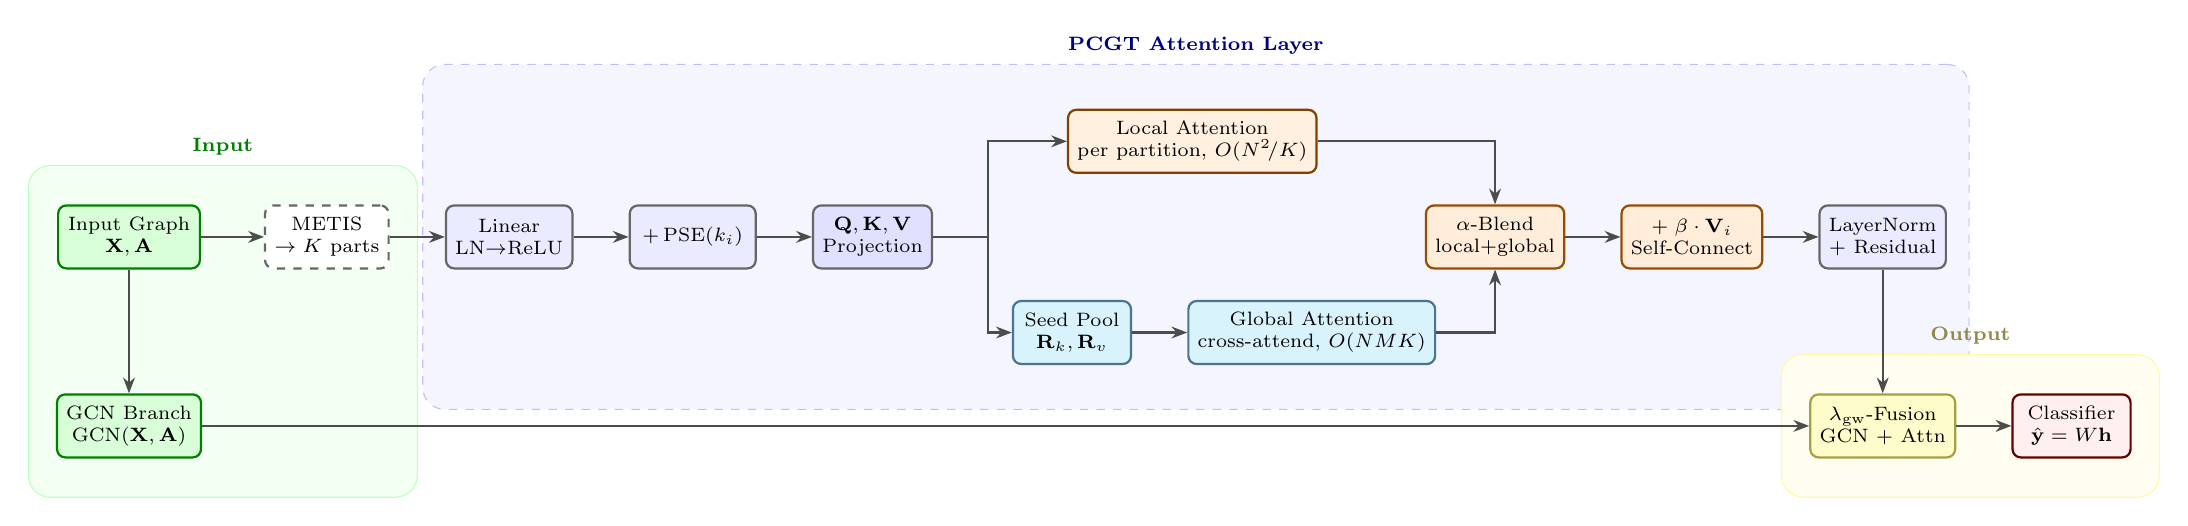
\begin{tikzpicture}[
  node distance=0.7cm and 0.8cm,
  box/.style={draw, rounded corners=3pt, minimum height=0.8cm, minimum width=1.5cm, align=center, font=\scriptsize},
  mainbox/.style={box, fill=white, draw=black!60, thick},
  gcnbox/.style={box, fill=green!15, draw=green!50!black, thick},
  fusebox/.style={box, fill=orange!15, draw=orange!60!black, thick},
  partbox/.style={box, fill=white, draw=black!60, thick, dashed, minimum width=1.2cm},
  localbox/.style={box, fill=orange!12, draw=orange!50!black, thick},
  globalbox/.style={box, fill=cyan!15, draw=cyan!50!black, thick},
  outbox/.style={box, fill=pink!25, draw=red!40!black, thick},
  arr/.style={-{Stealth[length=2mm]}, thick, black!70},
  stagelabel/.style={font=\scriptsize\bfseries, text=black!60},
]

% === Row 1: Main attention pipeline ===
% Input
\node[gcnbox, minimum width=1.8cm] (input) {Input Graph\\$\mathbf{X}, \mathbf{A}$};

% METIS
\node[partbox, right=0.8cm of input] (metis) {METIS\\$\to K$ parts};
\draw[arr] (input) -- (metis);

% Linear (applied first in code)
\node[mainbox, fill=blue!8, right=0.7cm of metis] (linproj) {Linear\\LN$\to$ReLU};
\draw[arr] (metis) -- (linproj);

% PSE (added after projection in code)
\node[mainbox, fill=blue!8, right=0.7cm of linproj, minimum width=1.6cm] (pse) {$+\,\text{PSE}(k_i)$};
\draw[arr] (linproj) -- (pse);

% QKV
\node[mainbox, fill=blue!12, right=0.7cm of pse] (qkv) {$\mathbf{Q,K,V}$\\Projection};
\draw[arr] (pse) -- (qkv);

% Fork point
\coordinate[right=0.7cm of qkv] (fork);
\draw[thick, black!70] (qkv) -- (fork);

% Local attention (top branch)
\node[localbox, above right=0.8cm and 1.0cm of fork] (local) {Local Attention\\per partition, $O(N^2\!/K)$};
\draw[arr] (fork) |- (local);

% Seed pool (bottom branch)
\node[globalbox, below right=0.8cm and 0.3cm of fork] (seedpool) {Seed Pool\\$\mathbf{R}_k, \mathbf{R}_v$};
\draw[arr] (fork) |- (seedpool);

% Global attention (right of seed pool)
\node[globalbox, right=0.7cm of seedpool] (global) {Global Attention\\cross-attend, $O(NMK)$};
\draw[arr] (seedpool) -- (global);

% Alpha-blend (centered right of the two branches)
\node[fusebox] (blend) at ($(local.east)!0.5!(global.east) + (1.5,0)$) {$\alpha$-Blend\\local$+$global};
\draw[arr] (local.east) -| (blend.north);
\draw[arr] (global.east) -| (blend.south);

% Self-connection
\node[fusebox, right=0.7cm of blend] (self) {$+\;\beta \cdot \mathbf{V}_i$\\Self-Connect};
\draw[arr] (blend) -- (self);

% LayerNorm
\node[mainbox, fill=blue!8, right=0.7cm of self] (ln) {LayerNorm\\$+$ Residual};
\draw[arr] (self) -- (ln);

% === Row 2: GCN branch ===
\node[gcnbox, minimum width=1.8cm] (gcn) at ($(input)+(0,-2.4)$) {GCN Branch\\$\text{GCN}(\mathbf{X,A})$};
\draw[arr] (input) -- (gcn);

% Fusion
\node[fusebox, fill=yellow!20, draw=yellow!60!black, minimum width=1.8cm] (gwfuse) at (ln |- gcn) {$\lambda_{\text{gw}}$-Fusion\\GCN $+$ Attn};
\draw[arr] (ln) -- (gwfuse);
\draw[arr] (gcn) -- (gwfuse);

% Output
\node[outbox, right=0.7cm of gwfuse, minimum width=1.5cm] (output) {Classifier\\$\hat{\mathbf{y}} = W\mathbf{h}$};
\draw[arr] (gwfuse) -- (output);

% === Background regions ===
\begin{scope}[on background layer]
  \node[fill=green!5, draw=green!25, rounded corners=8pt, inner xsep=10pt, inner ysep=14pt,
        fit=(input)(metis)(gcn),
        label={[stagelabel, text=green!50!black]above:Input}] {};
  \node[fill=blue!4, draw=blue!25, dashed, rounded corners=8pt, inner xsep=8pt, inner ysep=16pt,
        fit=(pse)(linproj)(qkv)(local)(global)(blend)(self)(ln)(seedpool),
        label={[stagelabel, text=blue!50!black]above:PCGT Attention Layer}] {};
  \node[fill=yellow!6, draw=yellow!35, rounded corners=8pt, inner xsep=10pt, inner ysep=14pt,
        fit=(gwfuse)(output),
        label={[stagelabel, text=yellow!50!black]above:Output}] {};
\end{scope}

\end{tikzpicture}
}% end resizebox
\caption{Architecture of PCGT. The input graph is partitioned via METIS into $K$ groups. Node features are linearly projected, augmented with partition structural encoding (PSE), then Q/K/V projections feed two parallel branches: \emph{local attention} within each partition (using Q, K, V restricted to the partition) and \emph{global attention} where learned seeds pool each partition's K, V into representatives $\mathbf{R}_k, \mathbf{R}_v$, and every node's Q cross-attends to all representatives. The branches are $\alpha$-blended, augmented with a $\beta$-weighted self-connection, and fused with a GCN branch via the graph-weight $\lambda_{\text{gw}}$.}
\label{fig:architecture}
\end{figure*}

PCGT combines local and global attention with learnable blending. Given a graph with $N$ nodes, we: (1) partition into $K$ regions (METIS/KMeans), (2) compute local attention within partitions $O(N^2/K)$, (3) compute global attention via learned seeds $O(N{\cdot}M{\cdot}K)$, (4) blend via learnable $\alpha$, (5) weight self-connections via learnable $\beta$, and (6) blend with GCN as fallback.

\subsection{Local Attention and Partition Encoding}

Partition the graph into $K$ disjoint sets $\{S_1, \ldots, S_K\}$ using METIS/KMeans, where $S_p \subset \{1,\ldots,N\}$ is the set of node indices in partition $p$. Given node features $\mathbf{X} \in \mathbb{R}^{N \times d}$, we compute query, key, and value projections $\mathbf{Q} = \mathbf{X} W_Q$, $\mathbf{K} = \mathbf{X} W_K$, $\mathbf{V} = \mathbf{X} W_V$ with learnable weights $W_Q, W_K, W_V \in \mathbb{R}^{d \times d}$. The notation $\mathbf{Q}[S_p] \in \mathbb{R}^{|S_p| \times d}$ selects the rows of $\mathbf{Q}$ corresponding to nodes in $S_p$ (likewise for $\mathbf{K}[S_p]$, $\mathbf{V}[S_p]$). Local attention within partition $p$ is:
\begin{equation}
\text{Attn}_{\text{local}}^{(p)} = \text{softmax}\!\left( \frac{\mathbf{Q}[S_p]\, \mathbf{K}[S_p]^T}{\sqrt{d}} \right) \mathbf{V}[S_p],\; O(N^2\!/K)
\end{equation}

Add partition structural encoding (PSE) before Q/K/V projection: $\mathbf{x}_i \leftarrow \mathbf{x}_i + \mathbf{E}_{k_i}$, where $\mathbf{E} \in \mathbb{R}^{K \times d}$ is a learned embedding table indexed by partition id $k_i$, initialized from $\mathcal{N}(0, 0.02)$.  PSE is added once (before projection) so that queries, keys, and values all encode partition membership.

\subsection{Global Attention via Learned Seeds}
\label{sec:global_attn}

We learn $M$ seed query vectors $\mathbf{S} \in \mathbb{R}^{M \times d}$ shared across all partitions. For each partition $p$, the seeds attention-pool the partition's keys and values into $M$ representative vectors. Let $\mathbf{A}_s^{(p)}$ denote the seed-to-partition attention weights:
\begin{equation}
\mathbf{A}_s^{(p)} = \mathrm{softmax}\!\left( \frac{\mathbf{S} \, \mathbf{K}[S_p]^T}{\sqrt{d}} \right) \in \mathbb{R}^{M \times |S_p|}
\label{eq:seed_attn}
\end{equation}
where $\mathbf{S} \in \mathbb{R}^{M \times d}$ are the learned seed queries, $\mathbf{K}[S_p] \in \mathbb{R}^{|S_p| \times d}$ are the key vectors of nodes in partition $p$, and $d$ is the hidden dimension. The softmax normalizes over the $|S_p|$ nodes in the partition, so each row of $\mathbf{A}_s^{(p)}$ is a distribution over partition members.

The key and value representatives are then:
\begin{align}
\mathbf{R}_k^{(p)} &= \mathbf{A}_s^{(p)} \, \mathbf{K}[S_p] \in \mathbb{R}^{M \times d} \label{eq:rk}\\
\mathbf{R}_v^{(p)} &= \mathbf{A}_s^{(p)} \, \mathbf{V}[S_p] \in \mathbb{R}^{M \times d} \label{eq:rv}
\end{align}
Here $\mathbf{V}[S_p] \in \mathbb{R}^{|S_p| \times d}$ are the value vectors of partition $p$. Each of the $M$ representatives is a weighted average of the partition's keys (resp.\ values), where the weights are determined by the learned seeds' attention over that partition's nodes. Stacking across all $K$ partitions yields $\mathbf{R}_k, \mathbf{R}_v \in \mathbb{R}^{KM \times d}$---a compact summary of the entire graph's keys and values. Each node then cross-attends to all representatives:
\begin{equation}
\text{Attn}_{\text{global}} = \text{softmax}\!\left( \frac{\mathbf{Q} \, \mathbf{R}_k^T}{\sqrt{d}} \right) \mathbf{R}_v, \quad O(N \!\cdot\! M \!\cdot\! K)
\end{equation}
where $\mathbf{Q} \in \mathbb{R}^{N \times d}$ are the query vectors of all $N$ nodes.
This two-step design (pool then cross-attend) is related to inducing points in Set Transformer~\citep{lee2019set}, but our seeds are \emph{topology-aware}: they pool from graph-partitioned node groups rather than arbitrary subsets, and adapt to the task unlike the fixed kernel in SGFormer~\citep{wu2023sgformer}.

\subsection{Blending, Self-Connection, and GCN Fusion}

The local and global outputs are blended with a learnable scalar $\alpha = \sigma(\alpha_{\text{logit}}) \in (0,1)$ where $\sigma$ is the sigmoid function:
\begin{equation}
\mathbf{h}_{\text{context}} = \alpha \cdot \text{Attn}_{\text{local}} + (1 - \alpha) \cdot \text{Attn}_{\text{global}}
\end{equation}
where $\text{Attn}_{\text{local}} \in \mathbb{R}^{N \times d}$ and $\text{Attn}_{\text{global}} \in \mathbb{R}^{N \times d}$ are the stacked local and global outputs from Eqs.~(1) and (5), and $\mathbf{h}_{\text{context}} \in \mathbb{R}^{N \times d}$ is the blended representation.

A learnable self-connection weight $\beta \in \mathbb{R}$ (unconstrained) adds the node's own transformed value:
\begin{equation}
\mathbf{h}_{\text{attn}} = \mathbf{h}_{\text{context}} + \beta \cdot \mathbf{V}_i
\end{equation}
where $\mathbf{V}_i \in \mathbb{R}^d$ is the value vector of node $i$ (the $i$-th row of $\mathbf{V}$).
Because $\beta$ is \emph{unconstrained}, it can become negative. On datasets where a node's own features are less informative than the attention context (e.g., Film, Deezer), this lets the model suppress the self-connection. Conversely, on feature-rich graphs like Chameleon and Squirrel, $\beta$ grows strongly positive. We formalize this: if the loss $\mathcal{L}$ is locally convex in $\beta$, then $\beta^* < 0$ whenever the self-features are, on aggregate, aligned with the loss-increasing direction (Proposition~\ref{prop:beta}, Appendix~\ref{app:beta_prop}).

Finally, the PCGT attention output is fused with a GCN branch via a fixed hyperparameter $\lambda_{\text{gw}} \in [0,1]$:
\begin{equation}
\mathbf{h}_{\text{final}} = \lambda_{\text{gw}} \cdot \text{GCN}(\mathbf{X}, \mathbf{A}) + (1 - \lambda_{\text{gw}}) \cdot \mathbf{h}_{\text{attn}}
\end{equation}
where $\mathbf{X} \in \mathbb{R}^{N \times d_{\text{in}}}$ is the input feature matrix, $\mathbf{A} \in \{0,1\}^{N \times N}$ is the adjacency matrix, and GCN is a standard multi-layer graph convolutional network~\citep{kipf2017semi}. The GCN branch provides explicit edge-level structural features that complement the partition-based attention.

The complete PCGT layer applies: input projection $\to$ partition structural encoding $\to$ Q,K,V projections $\to$ local + global attention $\to$ $\alpha$-blend $\to$ $\beta$ self-connection $\to$ LayerNorm $\to$ residual connection $\to$ dropout. The full procedure is summarized in Algorithm~\ref{alg:pcgt}.

\begin{algorithm}[t]
\caption{PCGT Forward Pass (one layer)}
\label{alg:pcgt}
\DontPrintSemicolon
\KwIn{Features $\mathbf{X} \in \mathbb{R}^{N \times d}$, adjacency $\mathbf{A}$, partitions $\{S_1, \ldots, S_K\}$}
\KwOut{Updated features $\mathbf{H} \in \mathbb{R}^{N \times d}$}
\BlankLine
$\mathbf{X} \leftarrow \mathbf{X} + \mathbf{E}[\text{partition id}]$ \tcp*{\color{gray}partition structural encoding}
$\mathbf{Q}, \mathbf{K}, \mathbf{V} \leftarrow \mathbf{X} W_Q,\; \mathbf{X} W_K,\; \mathbf{X} W_V$\;
\BlankLine
\For{$p = 1$ \KwTo $K$}{
  $\mathbf{h}^{(p)}_{\mathrm{local}} \leftarrow \mathrm{softmax}\!\bigl(\mathbf{Q}[S_p]\, \mathbf{K}[S_p]^{\!\top}\!/\sqrt{d}\bigr)\, \mathbf{V}[S_p]$\;
  $\mathbf{R}_k^{(p)},\, \mathbf{R}_v^{(p)} \leftarrow \mathrm{SeedPool}(\mathbf{S},\, \mathbf{K}[S_p],\, \mathbf{V}[S_p])$\;
}
Stack all $\mathbf{h}_{\mathrm{local}}^{(p)}$ into $\mathbf{h}_{\mathrm{local}} \!\in\! \mathbb{R}^{N \times d}$; all $\mathbf{R}_k^{(p)}, \mathbf{R}_v^{(p)}$ into $\mathbf{R}_k, \mathbf{R}_v \!\in\! \mathbb{R}^{KM \times d}$\;
$\mathbf{h}_{\mathrm{global}} \leftarrow \mathrm{softmax}\!\bigl(\mathbf{Q}\, \mathbf{R}_k^{\!\top}\!/\sqrt{d}\bigr)\, \mathbf{R}_v$ \tcp*{\color{gray}global cross-attention}
\BlankLine
$\mathbf{h}_{\mathrm{ctx}} \leftarrow \sigma(\alpha)\, \mathbf{h}_{\mathrm{local}} + (1\!-\!\sigma(\alpha))\, \mathbf{h}_{\mathrm{global}}$\;
$\mathbf{h}_{\mathrm{attn}} \leftarrow \mathbf{h}_{\mathrm{ctx}} + \beta \cdot \mathbf{V}$ \tcp*{\color{gray}self-connection}
$\mathbf{H} \leftarrow \lambda_{\mathrm{gw}}\, \mathrm{GCN}(\mathbf{X}, \mathbf{A}) + (1\!-\!\lambda_{\mathrm{gw}})\, \mathrm{LN}(\mathbf{h}_{\mathrm{attn}})$\;
\Return{$\mathbf{H}$}
\end{algorithm}

\subsection{Complexity}

Total per layer: $O(N^2/K + NMK + |E|)$. For $N$=10K--100K, $K$=50, $M$=4: PCGT achieves $\sim$3M--220M ops vs.\ $\sim$100M--10B for standard $O(N^2)$ attention.

\subsection{Connection to Nystr\"om Attention}
\label{sec:nystrom}

The effective attention in PCGT admits a structured factorization that connects to the Nystr\"om approximation of kernel matrices~\citep{xiong2021nystromformer}.

\begin{remark}[Attention Factorization]
The PCGT attention matrix decomposes as:
\begin{equation}
\boldsymbol{\Omega}_{\mathrm{PCGT}} = \alpha \cdot \boldsymbol{\Omega}_{\mathrm{local}} + (1-\alpha) \cdot \boldsymbol{\Omega}_{\mathrm{global}}
\label{eq:factorization}
\end{equation}
where $\boldsymbol{\Omega}_{\mathrm{local}} \in \mathbb{R}^{N \times N}$ is \emph{block-diagonal} (exact softmax attention within each partition) and $\boldsymbol{\Omega}_{\mathrm{global}}$ admits a \emph{low-rank factorization}:
\begin{equation}
\boldsymbol{\Omega}_{\mathrm{global}} = \mathbf{P} \cdot \mathbf{W} \quad \text{with}\; \mathbf{P} \in \mathbb{R}^{N \times KM},\; \mathbf{W} \in \mathbb{R}^{KM \times N}
\label{eq:lowrank}
\end{equation}
where $P_{i,m} = \mathrm{softmax}(\mathbf{q}_i^T \mathbf{r}_k^{(m)} / \sqrt{d})$ is node $i$'s attention to representative $m$, and $W_{m,j} = \mathrm{softmax}(\mathbf{s}^T \mathbf{k}_j / \sqrt{d})$ is representative $m$'s pooling weight on node $j$.
\end{remark}

This structure is analogous to the Nystr\"om method, where a kernel matrix is approximated via a small set of \emph{landmark} columns: $\mathbf{K} \approx \mathbf{K}_{N,m} \mathbf{K}_{m,m}^{-1} \mathbf{K}_{m,N}$. In PCGT, the $KM$ partition representatives serve as topology-aware landmarks. The analogy is structural, not exact: Nystr\"om uses an explicit inverse $\mathbf{K}_{m,m}^{-1}$ for reconstruction, whereas PCGT's $\mathbf{P}$ and $\mathbf{W}$ are independently softmax-normalized, making the factorization a learned low-rank approximation rather than an analytical one.  Unlike generic Nystr\"om methods (e.g., Nystr\"omformer~\citep{xiong2021nystromformer}), which sample or hash random columns, PCGT's landmarks are \emph{graph-structure-aware}: they are produced by attention-pooling within METIS partitions, so the low-rank component respects the graph's community structure.

The full PCGT attention thus combines a \emph{high-rank block-diagonal} component (capturing intra-community detail) with a \emph{low-rank global} component (capturing cross-community interactions)---a spectral complement where the local term covers within-partition frequencies and the global term covers between-partition frequencies. This is why a single PCGT layer can be both expressive and subquadratic.




% ============================================================================
% EXPERIMENTS
% ============================================================================
\section{Experiments}

\subsection{Datasets}

We evaluate on 14 node classification benchmarks spanning homophilic, heterophilic, and large-scale regimes, following the dataset selection and preprocessing of SGFormer~\citep{wu2023sgformer} and extending to standard co-purchase, co-authorship~\citep{shchur2018pitfalls}, and OGB~\citep{hu2020ogb} datasets. Dataset statistics are summarized in Table~\ref{tab:datasets}.

\begin{table}[t]
\centering
\small
\resizebox{\columnwidth}{!}{%
\begin{tabular}{lrrrrr}
\toprule
\textbf{Dataset} & \textbf{Nodes} & \textbf{Feats} & \textbf{Classes} & \textbf{$h$} & \textbf{Type} \\
\midrule
Cora       & 2,708  & 1,433  & 7  & 0.81 & Homo. \\
CiteSeer   & 3,327  & 3,703  & 6  & 0.74 & Homo. \\
PubMed     & 19,717 & 500    & 3  & 0.80 & Homo. \\
Coauthor-CS & 18,333 & 6,805 & 15 & 0.81 & Homo. \\
Coauthor-Phys. & 34,493 & 8,415 & 5 & 0.93 & Homo. \\
Amazon-Comp. & 13,752 & 767  & 10 & 0.78 & Homo. \\
Amazon-Photo & 7,650  & 745   & 8  & 0.83 & Homo. \\
Chameleon  & 890    & 2,325  & 5  & 0.24 & Hetero. \\
Film       & 7,600  & 932    & 5  & 0.22 & Hetero. \\
Squirrel   & 2,223  & 2,089  & 5  & 0.21 & Hetero. \\
Deezer     & 28,281 & 31,241 & 2  & 0.53 & Mixed \\
\midrule
ogbn-arxiv & 169,343 & 128 & 40 & 0.66 & Large \\
pokec      & 1,632,803 & 65 & 2 & 0.45 & Large \\
Amazon2M   & 2,449,029 & 100 & 47 & 0.78 & Large \\
\bottomrule
\end{tabular}
}% end resizebox
\caption{Dataset statistics. $h$ denotes edge homophily ratio. Chameleon and Squirrel use filtered splits from~\citet{platonov2023critical}.}
\label{tab:datasets}
\end{table}

\noindent\textbf{Homophilic benchmarks.} Cora, CiteSeer, and PubMed are standard citation networks~\citep{kipf2017semi, sen2008collective} where connected nodes tend to share labels. Coauthor-CS and Coauthor-Physics are co-authorship graphs~\citep{shchur2018pitfalls} where nodes represent authors. Amazon-Computers and Amazon-Photo are co-purchase graphs from the Amazon product network~\citep{shchur2018pitfalls}.
\textbf{Heterophilic benchmarks.} Chameleon and Squirrel are Wikipedia page--page networks with filtered splits from \citet{platonov2023critical}, where edges frequently connect nodes of different classes. Film is an actor co-occurrence network~\citep{pei2020geomgcn}. \textbf{Deezer}~\citep{rozemberczki2021deezer} is a social network with binary genre labels and mixed homophily.
\textbf{ogbn-arxiv}~\citep{hu2020ogb} is a large-scale citation network (169K nodes, 1.2M edges, 40 classes) from the Open Graph Benchmark.
\textbf{pokec}~\citep{lim2021large} is a social network (1.6M nodes, 30.6M edges) with binary gender labels and heterophilic structure ($h$=0.45), using 10\%/10\%/80\% random splits.
\textbf{Amazon2M}~\citep{wu2022nodeformer} is a co-purchasing network (2.4M nodes, 61.9M edges, 47 classes) with bag-of-words features, using 50\%/25\%/25\% random splits.

\subsection{Evaluation Protocol}

We follow the identical evaluation protocol of SGFormer~\citep{wu2023sgformer} to enable direct comparison:

\begin{itemize}
    \item \textbf{Cora, CiteSeer, PubMed:} Semi-supervised setting with 20 labels per class, 500 validation nodes, and 1000 test nodes (random class-balanced splits). 10 runs.
    \item \textbf{Coauthor-CS, Coauthor-Physics, Amazon-Computers, Amazon-Photo:} Random 50\%/25\%/25\% splits. 10 runs.
    \item \textbf{Chameleon, Squirrel, Film:} Pre-computed 10-fold filtered splits (60\%/20\%/20\%) from~\citet{platonov2023critical}. 10 runs.
    \item \textbf{Deezer:} Random 50\%/25\%/25\% splits. 10 runs.
    \item \textbf{ogbn-arxiv:} Official OGB train/val/test split~\citep{hu2020ogb}. 10 runs.
    \item \textbf{pokec:} Random 10\%/10\%/80\% split~\citep{lim2021large}. 3 runs.
    \item \textbf{Amazon2M:} Random 50\%/25\%/25\% split~\citep{wu2022nodeformer}. 3 runs.
\end{itemize}

We report mean $\pm$ standard deviation of the highest test accuracy observed during training across runs. Early stopping uses patience 200 on validation accuracy. This metric follows the SGFormer evaluation protocol: both codebases use identical \texttt{logger.py} code that records the peak test accuracy across all epochs.

\subsection{Baselines}

We compare against 13 methods spanning three categories: (1)~\emph{Standard GNNs}: GCN~\citep{kipf2017semi}, GAT~\citep{velickovic2018gat}, APPNP~\citep{klicpera2019appnp}, SIGN~\citep{rossi2020sign}; (2)~\emph{Heterophily-specific GNNs}: H$_2$GCN~\citep{zhu2020h2gcn}, CPGNN~\citep{zhu2021cpgnn}, GloGNN~\citep{li2022glognn}; (3)~\emph{Graph Transformers}: NodeFormer~\citep{wu2022nodeformer}, DIFFormer~\citep{wu2023difformer}, NAGphormer~\citep{chen2023nagphormer}, GraphGPS~\citep{rampasek2022graphgps}, SGFormer~\citep{wu2023sgformer}. Baseline results for the original 7 datasets are taken from \citet{wu2023sgformer}, Table~2; GraphGPS results are from our own runs using the Performer-attention variant~\citep{rampasek2022graphgps} under the same splits and evaluation protocol. For Coauthor and Amazon datasets, SGFormer baselines are from our own runs with identical code and hyperparameters.

\noindent\textbf{Note on Exphormer.}~~Exphormer~\citep{shirzad2023exphormer} primarily benchmarks on \emph{graph-level} tasks (ZINC, LRGB) and does not report node classification results under the semi-supervised protocol we follow. We discuss its architectural relationship to PCGT in Section~\ref{sec:nystrom} and Related Work.

\subsection{Implementation Details}

\textbf{Architecture.} PCGT uses hidden dimension $d=64$, 1 PCGT attention layer ($L_\text{pcgt}=1$), $M=4$ learned seeds per partition, and a multi-layer GCN backbone ($L_\text{gcn} \in \{2, 4\}$ depending on dataset). The GCN branch uses residual connections. Partition structural encoding (PSE) adds a learned $K \times d$ embedding to node features at each PCGT layer. We fix $M=4$ across all experiments; accuracy is stable across $M \in \{2, 4, 8\}$, with differences within noise (Appendix Table~\ref{tab:m_ablation}).

\textbf{Partitioning.} We compute METIS~\citep{karypis1998metis} partitions once on the full graph adjacency before training. This is consistent with the transductive setting: all methods (GCN, GAT, SGFormer) access the full graph structure---including test-node edges---during message passing. PCGT uses the same structural information, organized through partitions rather than direct neighbor aggregation. The number of partitions $K$ is tuned per dataset: $K=10$ for Cora/Chameleon/Squirrel, $K=20$ for CiteSeer/Deezer, $K=50$ for PubMed, and $K=5$ for Film.

\textbf{Optimization.} Adam optimizer~\citep{kingma2015adam} with learning rate 0.01 (0.05 for Film). We apply differential weight decay: a base weight decay for the GCN branch and a separate weight decay for the PCGT attention parameters. Dropout rates are tuned per dataset in $\{0.2, 0.3, 0.4, 0.5, 0.7\}$, with heavier regularization for larger or noisier datasets.

\textbf{Hyperparameter selection.} All hyperparameters were selected via grid search on the validation set. For each dataset, we searched $K \in \{5, 10, 15, 20, 30, 50\}$, $\lambda_{\text{gw}} \in \{0.5, 0.7, 0.8\}$, dropout $\in \{0.2, 0.3, 0.4, 0.5, 0.7\}$, and weight decay $\in \{5\text{e-}5, 5\text{e-}4, 1\text{e-}3, 1\text{e-}2\}$, selecting the configuration with the highest mean validation accuracy over 3 preliminary runs. The final results are reported with 10 runs using the selected configuration.

\textbf{Key hyperparameters.} The graph weight $\lambda_{\text{gw}} \in \{0.5, 0.7, 0.8\}$ controls the GCN vs.\ PCGT attention blend. On homophilic graphs, $\lambda_{\text{gw}}=0.8$ favors the GCN branch; on heterophilic or mixed-homophily graphs, lower values (0.5) increase the PCGT contribution. The local--global blend $\alpha$ and self-connection weight $\beta$ are learned end-to-end, initialized at 0.5 and 1.0 respectively.

\subsection{Ablation Study}
\label{sec:ablation}

To validate that each component of PCGT contributes to performance, we conduct ablations on three representative datasets: Cora (homophilic), Chameleon (heterophilic), and Squirrel (heterophilic). We test the following variants:

\begin{enumerate}
    \item \textbf{w/o Global attention} (\texttt{local\_only}): Remove the cross-partition seed-based attention; only intra-partition attention is used.
    \item \textbf{w/o Local attention} (\texttt{global\_only}): Remove intra-partition attention; only cross-partition global attention via learned seeds.
    \item \textbf{w/o PSE} (\texttt{no\_pse}): Remove partition structural encoding, so the model receives no explicit signal about partition membership.
    \item \textbf{w/o GCN branch}: Set $\text{gw}=0$ and disable the GCN backbone, testing pure PCGT attention.
    \item \textbf{Random partitions}: Replace METIS with random node assignment, testing whether topology-aware partitioning matters.
    \item \textbf{K sweep}: Vary $K \in \{5, 10, 15, 20, 30\}$ on Chameleon and Squirrel to study the effect of partition granularity.
\end{enumerate}

\noindent Results are reported in Section~\ref{sec:results}.


% ============================================================================
% RESULTS
% ============================================================================
\section{Results}
\label{sec:results}

\subsection{Main Performance}

Table~\ref{tab:main} compares PCGT against 13 baselines on 7 medium-scale datasets. Baseline results for GCN through SGFormer are taken from \citet{wu2023sgformer}; DIFFormer from \citet{wu2023difformer}; NAGphormer from \citet{chen2023nagphormer}; GraphGPS from our own runs using the Performer-attention implementation of \citet{rampasek2022graphgps}. PCGT numbers are from our own runs on an NVIDIA H100 GPU (10 runs each).

\begin{table*}[t]
\centering
\small
\setlength{\tabcolsep}{3pt}
\resizebox{\textwidth}{!}{%
\begin{tabular}{l|ccc|cccc}
\toprule
 & \multicolumn{3}{c|}{\textbf{Homophilic}} & \multicolumn{4}{c}{\textbf{Heterophilic}} \\
\textbf{Method} & \textbf{Cora} & \textbf{CiteSeer} & \textbf{PubMed} & \textbf{Film} & \textbf{Squirrel} & \textbf{Chameleon} & \textbf{Deezer} \\
\midrule
\multicolumn{8}{l}{\textit{Standard GNNs}} \\
GCN & 81.6{\scriptsize$\pm$0.4} & 71.6{\scriptsize$\pm$0.4} & 78.8{\scriptsize$\pm$0.6} & 30.1{\scriptsize$\pm$0.2} & 38.6{\scriptsize$\pm$1.8} & 41.3{\scriptsize$\pm$3.0} & 62.7{\scriptsize$\pm$0.7} \\
GAT & 83.0{\scriptsize$\pm$0.7} & 72.1{\scriptsize$\pm$1.1} & 79.0{\scriptsize$\pm$0.4} & 29.8{\scriptsize$\pm$0.6} & 35.6{\scriptsize$\pm$2.1} & 39.2{\scriptsize$\pm$3.1} & 61.7{\scriptsize$\pm$0.8} \\
APPNP & 83.3{\scriptsize$\pm$0.5} & 71.8{\scriptsize$\pm$0.5} & 80.1{\scriptsize$\pm$0.2} & 31.3{\scriptsize$\pm$1.5} & 35.3{\scriptsize$\pm$1.9} & 38.4{\scriptsize$\pm$3.5} & 66.1{\scriptsize$\pm$0.6} \\
SIGN & 82.1{\scriptsize$\pm$0.3} & 72.4{\scriptsize$\pm$0.8} & 79.5{\scriptsize$\pm$0.5} & 36.5{\scriptsize$\pm$1.0} & 40.7{\scriptsize$\pm$2.5} & 41.7{\scriptsize$\pm$2.2} & 66.3{\scriptsize$\pm$0.3} \\
\midrule
\multicolumn{8}{l}{\textit{Heterophily-Specific GNNs}} \\
H$_2$GCN & 82.5{\scriptsize$\pm$0.8} & 71.4{\scriptsize$\pm$0.7} & 79.4{\scriptsize$\pm$0.4} & 34.4{\scriptsize$\pm$1.7} & 35.1{\scriptsize$\pm$1.2} & 38.1{\scriptsize$\pm$4.0} & 66.2{\scriptsize$\pm$0.8} \\
CPGNN & 80.8{\scriptsize$\pm$0.4} & 71.6{\scriptsize$\pm$0.4} & 78.5{\scriptsize$\pm$0.7} & 34.5{\scriptsize$\pm$0.7} & 38.9{\scriptsize$\pm$1.2} & 40.8{\scriptsize$\pm$2.0} & 65.8{\scriptsize$\pm$0.3} \\
GloGNN & 81.9{\scriptsize$\pm$0.4} & 72.1{\scriptsize$\pm$0.6} & 78.9{\scriptsize$\pm$0.4} & 36.4{\scriptsize$\pm$1.6} & 35.7{\scriptsize$\pm$1.3} & 40.2{\scriptsize$\pm$3.9} & 65.8{\scriptsize$\pm$0.8} \\
\midrule
\multicolumn{8}{l}{\textit{Graph Transformers}} \\
NodeFormer & 82.2{\scriptsize$\pm$0.9} & 72.5{\scriptsize$\pm$1.1} & 79.9{\scriptsize$\pm$1.0} & 36.9{\scriptsize$\pm$1.0} & 38.5{\scriptsize$\pm$1.5} & 34.7{\scriptsize$\pm$4.1} & 66.4{\scriptsize$\pm$0.7} \\
DIFFormer & 83.5{\scriptsize$\pm$0.6} & 72.2{\scriptsize$\pm$0.5} & 79.7{\scriptsize$\pm$0.6} & 37.5{\scriptsize$\pm$1.0} & 39.5{\scriptsize$\pm$2.1} & 44.0{\scriptsize$\pm$3.5} & 66.4{\scriptsize$\pm$0.9} \\
NAGphormer & 83.2{\scriptsize$\pm$0.8} & 72.3{\scriptsize$\pm$0.4} & 78.6{\scriptsize$\pm$0.3} & 35.8{\scriptsize$\pm$1.1} & 38.3{\scriptsize$\pm$1.9} & 42.3{\scriptsize$\pm$3.1} & 66.7{\scriptsize$\pm$0.7} \\
GraphGPS & 78.6{\scriptsize$\pm$1.7} & 60.4{\scriptsize$\pm$1.4} & 75.5{\scriptsize$\pm$0.7} & 34.0{\scriptsize$\pm$0.6} & 36.5{\scriptsize$\pm$2.5} & 44.2{\scriptsize$\pm$3.5} & 67.0{\scriptsize$\pm$0.7} \\
SGFormer & \best{84.5}{\scriptsize$\pm$0.8} & \runup{72.6}{\scriptsize$\pm$0.2} & \runup{80.3}{\scriptsize$\pm$0.6} & \runup{37.9}{\scriptsize$\pm$1.1} & \runup{41.8}{\scriptsize$\pm$2.2} & \runup{44.9}{\scriptsize$\pm$3.9} & \runup{67.1}{\scriptsize$\pm$1.1} \\
\midrule
\textbf{PCGT (ours)} & \runup{84.3}{\scriptsize$\pm$0.4} & \best{73.1}{\scriptsize$\pm$0.4} & \best{81.0}{\scriptsize$\pm$0.6} & \best{38.0}{\scriptsize$\pm$0.9} & \best{45.5}{\scriptsize$\pm$2.7} & \best{49.0}{\scriptsize$\pm$2.8} & \best{67.2}{\scriptsize$\pm$0.7} \\
\bottomrule
\end{tabular}
}% end resizebox
\caption{Node classification accuracy (\%) on medium-scale benchmarks. Mean $\pm$ std over 10 runs (Deezer: 5 runs). GCN--SGFormer from \citet{wu2023sgformer}; DIFFormer from \citet{wu2023difformer}; NAGphormer from \citet{chen2023nagphormer}; GraphGPS from our runs. \best{Best} and \runup{runner-up} per column.}
\label{tab:main}
\end{table*}

Table~\ref{tab:new_datasets} reports results on four additional datasets where we run both SGFormer and PCGT under identical settings (10 runs each, random 50/25/25 splits).

\begin{table}[t]
\centering
\small
\setlength{\tabcolsep}{3pt}
\resizebox{\columnwidth}{!}{%
\begin{tabular}{l|cccc}
\toprule
\textbf{Method} & \textbf{Co-CS} & \textbf{Co-Phys} & \textbf{Am-Comp} & \textbf{Am-Photo} \\
\midrule
GCN & 91.9{\scriptsize$\pm$0.4} & 95.7{\scriptsize$\pm$0.2} & 82.8{\scriptsize$\pm$1.8} & 90.9{\scriptsize$\pm$1.2} \\
GAT & 92.0{\scriptsize$\pm$0.3} & 95.4{\scriptsize$\pm$0.2} & 83.4{\scriptsize$\pm$0.9} & 91.1{\scriptsize$\pm$0.8} \\
SGFormer & \runup{94.9}{\scriptsize$\pm$0.5} & \runup{96.6}{\scriptsize$\pm$0.2} & \runup{87.5}{\scriptsize$\pm$2.0} & \runup{95.2}{\scriptsize$\pm$1.2} \\
\textbf{PCGT (ours)} & \best{95.1}{\scriptsize$\pm$0.3} & \best{96.8}{\scriptsize$\pm$0.2} & \best{88.8}{\scriptsize$\pm$0.7} & \best{95.3}{\scriptsize$\pm$0.4} \\
\bottomrule
\end{tabular}}%
\caption{Accuracy (\%) on four additional datasets. Mean $\pm$ std over 10 runs. GCN and GAT baselines from our own runs on H100. \best{Best} and \runup{runner-up} per column.}
\label{tab:new_datasets}
\end{table}

\textbf{Heterophilic datasets.} The largest gains are on heterophilic benchmarks: +4.1\% on Chameleon and +3.7\% on Squirrel over SGFormer, which was already the previous best. PCGT beats all 13 baselines on these datasets, including heterophily-specific methods like GloGNN (+8.8\% on Chameleon) and H$_2$GCN (+10.4\% on Squirrel). On Film, PCGT also leads (38.0 vs.\ 37.9 for SGFormer).

\textbf{Homophilic datasets.} On CiteSeer, PCGT scores 73.1 vs.\ SGFormer's 72.6 (+0.5\%). On PubMed, 81.0 vs.\ 80.3 (+0.7\%). On Cora, the two are within noise (84.3 vs.\ 84.5). PCGT also shows lower run-to-run variance than SGFormer across these benchmarks.

\textbf{Additional datasets (Table~\ref{tab:new_datasets}).} PCGT wins on all four, outperforming not only SGFormer but also GCN and GAT baselines by large margins. Coauthor-Physics (+0.2\% over SGFormer) is statistically significant ($p$=0.004). Amazon-Computers has the largest absolute gap (+1.3\%, $p$=0.051). PCGT's variance is also consistently lower (e.g., $\pm$0.7 vs.\ $\pm$2.0 on Amazon-Computers).

\textbf{Mixed homophily (Deezer).} PCGT scores 67.2 vs.\ SGFormer's 67.1 on Deezer ($h \approx 0.5$), a +0.1\% gap that is within the error bars and not statistically significant. With a lower graph weight ($\lambda_{\text{gw}}=0.5$), PCGT gives more influence to the partition-conditioned attention, but the gain on this mixed-homophily dataset is marginal.

\subsection{Large-Scale Results}

To test scalability beyond medium-sized graphs, we evaluate on three large-scale benchmarks spanning homophilic and heterophilic regimes: ogbn-arxiv (169K nodes, 1.2M edges)~\citep{hu2020ogb}, pokec (1.6M nodes, 30.6M edges)~\citep{lim2021large}, and Amazon2M (2.4M nodes, 61.9M edges)~\citep{wu2022nodeformer}. We follow the mini-batch training setup of SGFormer~\citep{wu2023sgformer}. Baselines are from \citet{wu2023sgformer} Table~3.

\begin{table}[t]
\centering
\small
\resizebox{\columnwidth}{!}{%
\begin{tabular}{l|ccc}
\toprule
\textbf{Method} & \textbf{ogbn-arxiv} & \textbf{pokec} & \textbf{Amazon2M} \\
\midrule
MLP & 55.50{\scriptsize$\pm$0.23} & 60.15{\scriptsize$\pm$0.03} & 63.46{\scriptsize$\pm$0.10} \\
GCN~\citep{kipf2017semi} & 71.74{\scriptsize$\pm$0.29} & 62.31{\scriptsize$\pm$1.13} & 83.90{\scriptsize$\pm$0.10} \\
SIGN~\citep{rossi2020sign} & 71.95{\scriptsize$\pm$0.11} & 68.01{\scriptsize$\pm$0.25} & 80.98{\scriptsize$\pm$0.31} \\
NodeFormer~\citep{wu2022nodeformer} & 59.90{\scriptsize$\pm$0.42} & 70.32{\scriptsize$\pm$0.45} & 87.85{\scriptsize$\pm$0.24} \\
SGFormer~\citep{wu2023sgformer} & \best{72.63}{\scriptsize$\pm$0.13} & 73.76{\scriptsize$\pm$0.24} & \best{89.09}{\scriptsize$\pm$0.10} \\
\midrule
\textbf{PCGT (ours)} & \runup{72.50}{\scriptsize$\pm$0.14} & \best{74.94}{\scriptsize$\pm$0.28} & \runup{88.79}{\scriptsize$\pm$0.06} \\
\bottomrule
\end{tabular}
}% end resizebox
\caption{Large-scale node classification accuracy (\%). Baselines from~\citet{wu2023sgformer} Table~3. PCGT: 10 runs (arxiv), 3 runs (pokec, Amazon2M), best validation epoch.}
\label{tab:largescale}
\end{table}

\noindent PCGT achieves the best result on pokec (74.94\%, +1.2\% over SGFormer) and is runner-up on ogbn-arxiv (72.50\% vs.\ 72.63\%) and Amazon2M (88.79\% vs.\ 89.09\%), both within the error bars of SGFormer. On pokec---a heterophilic social network ($h$=0.45) with 1.6M nodes---partition-conditioned attention provides meaningful gains, consistent with the pattern observed on medium-scale heterophilic graphs. On homophilic graphs (arxiv $h$=0.66, Amazon2M), SGFormer's lightweight $O(N)$ kernel is well-suited, so matching it is the expected outcome. Importantly, PCGT scales to 2.4M nodes without accuracy collapse, confirming that $O(N^2/K + NMK)$ complexity remains practical at million-node scale.

\begin{figure}[t]
\centering
\resizebox{\columnwidth}{!}{%
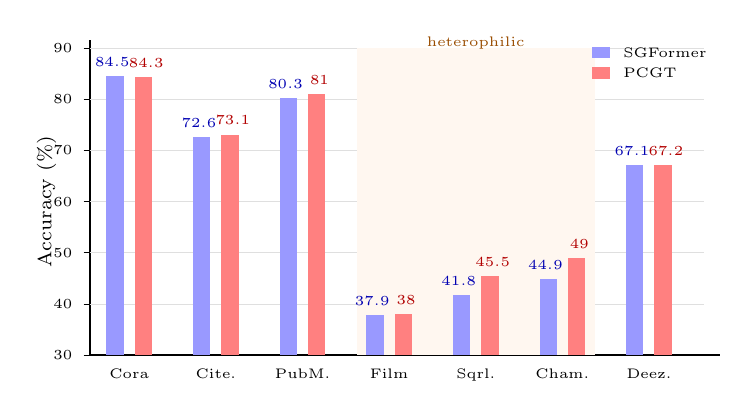
\begin{tikzpicture}[
  every node/.style={font=\scriptsize},
]
\pgfmathsetmacro{\bw}{0.22}  % bar width in cm
\pgfmathsetmacro{\gap}{0.14} % gap between paired bars
\pgfmathsetmacro{\sp}{1.1}   % spacing between groups

% Data: SGFormer and PCGT accuracies
% Cora 84.5/84.3, CiteSeer 72.6/73.1, PubMed 80.3/81.0, Film 37.9/38.0, Squirrel 41.8/45.5, Cham 44.9/49.0, Deezer 67.1/67.2

% Y-axis: show from 30 to 90, scale factor
\pgfmathsetmacro{\ymin}{30}
\pgfmathsetmacro{\yscale}{0.065}

% Draw axes
\draw[thick] (0,0) -- (0,{(90-\ymin)*\yscale+0.1});
\draw[thick] (0,0) -- ({7*\sp+0.3},0);

% Y-axis ticks and labels
\foreach \y/\lab in {30/30, 40/40, 50/50, 60/60, 70/70, 80/80, 90/90} {
  \draw (-0.08,{(\y-\ymin)*\yscale}) -- (0,{(\y-\ymin)*\yscale});
  \node[left, font=\tiny] at (-0.1,{(\y-\ymin)*\yscale}) {\lab};
}
% Y-axis label
\node[rotate=90, font=\scriptsize] at (-0.55,{(60-\ymin)*\yscale}) {Accuracy (\%)};

% Gridlines
\foreach \y in {40,50,60,70,80,90} {
  \draw[gray!25, thin] (0,{(\y-\ymin)*\yscale}) -- ({7*\sp+0.1},{(\y-\ymin)*\yscale});
}

% Heterophilic background zone (behind bars, subtle)
\fill[orange!6] ({3*\sp+0.5-\bw-\gap/2-0.12},0) rectangle ({5*\sp+0.5+\bw+\gap/2+0.12},{(90-\ymin)*\yscale});
\node[font=\tiny, orange!60!black] at ({4*\sp+0.5},{(91-\ymin)*\yscale}) {heterophilic};

% Bar data: {index}{label}{sgf_val}{pcgt_val}
\foreach \i/\lab/\sgf/\pcgt in {
  0/Cora/84.5/84.3,
  1/Cite./72.6/73.1,
  2/PubM./80.3/81.0,
  3/Film/37.9/38.0,
  4/Sqrl./41.8/45.5,
  5/Cham./44.9/49.0,
  6/Deez./67.1/67.2%
} {
  \pgfmathsetmacro{\xc}{\i*\sp+0.5}
  % SGFormer bar (blue)
  \fill[blue!40] ({\xc-\bw-\gap/2},0) rectangle ({\xc-\gap/2},{(\sgf-\ymin)*\yscale});
  % PCGT bar (red/orange)
  \fill[red!50] ({\xc+\gap/2},0) rectangle ({\xc+\bw+\gap/2},{(\pcgt-\ymin)*\yscale});
  % Value labels — offset left/right to avoid overlap
  \node[above, font=\tiny, blue!70!black, xshift=-1pt] at ({\xc-\bw/2-\gap/2},{(\sgf-\ymin)*\yscale}) {\pgfmathprintnumber[fixed, precision=1]{\sgf}};
  \node[above, font=\tiny, red!70!black, xshift=1pt] at ({\xc+\bw/2+\gap/2},{(\pcgt-\ymin)*\yscale}) {\pgfmathprintnumber[fixed, precision=1]{\pcgt}};
  % X-axis label
  \node[below, font=\tiny] at ({\xc},-0.05) {\lab};
}

% Legend
\fill[blue!40] ({5.8*\sp},  {(88-\ymin)*\yscale}) rectangle +(\bw,0.15);
\node[right, font=\tiny] at ({5.8*\sp+\bw+0.05},{(88-\ymin)*\yscale+0.075}) {SGFormer};
\fill[red!50]  ({5.8*\sp},  {(84-\ymin)*\yscale}) rectangle +(\bw,0.15);
\node[right, font=\tiny] at ({5.8*\sp+\bw+0.05},{(84-\ymin)*\yscale+0.075}) {PCGT};

\end{tikzpicture}
}% end resizebox
\caption{PCGT vs.\ SGFormer accuracy across all 7 datasets. PCGT shows the largest gains on heterophilic benchmarks (shaded), particularly Chameleon (+4.1\%) and Squirrel (+3.7\%).}
\label{fig:comparison}
\end{figure}

\subsection{Learned Parameters}

Analysis of the learned $\alpha$ and $\beta$ values reveals adaptive behavior:
\begin{itemize}
\item $\alpha$ (local vs.~global blend) stabilizes near 0.5 across datasets, indicating that both local and global attention contribute roughly equally with the current single-layer design.
\item $\beta$ (self-connection) is dataset-dependent and \emph{unconstrained}. On 9 of 11 datasets $\beta > 0$ (the model amplifies self-features), with the largest values on Squirrel ($\beta = +3.53$) and Chameleon ($\beta = +3.08$)---datasets with high-dimensional features (2089 and 2325 dims) where self-identity is highly informative. On Film ($\beta = -0.99 \pm 1.43$, negative in 8/10 splits) and Deezer ($\beta = -0.57 \pm 0.25$, negative in 5/5 runs), the model suppresses self-features. Notably, there is no linear correlation between $\beta$ and homophily (Pearson $r = 0.006$, $p = 0.99$ across all 11 datasets), suggesting that $\beta$ may reflect complementarity between self-features and attention-weighted context rather than homophily per se (though with only 11 datasets, this correlation test has limited statistical power).
\end{itemize}

\begin{figure}[t]
\centering
\resizebox{\columnwidth}{!}{%
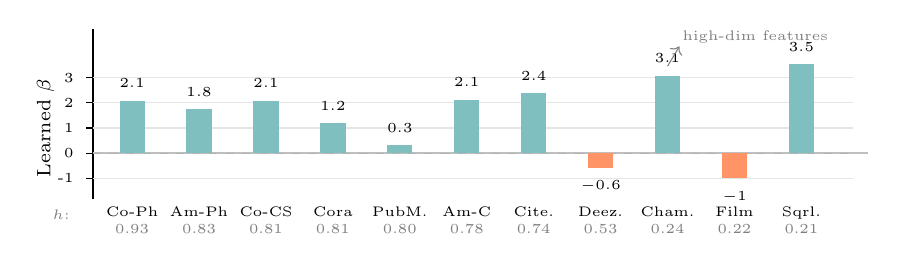
\begin{tikzpicture}[every node/.style={font=\scriptsize}]
\pgfmathsetmacro{\bw}{0.32}
\pgfmathsetmacro{\sp}{0.85}
\pgfmathsetmacro{\yscale}{0.32}

% Axes
\draw[thick] (0,-1.5*\yscale-0.1) -- (0,4.0*\yscale+0.3);
\draw[thick, gray!50] (0,0) -- ({11*\sp+0.5},0);

% Y ticks
\foreach \y in {-1,0,1,2,3} {
  \draw (-0.08,{\y*\yscale}) -- (0,{\y*\yscale});
  \node[left, font=\tiny] at (-0.12,{\y*\yscale}) {\y};
}
\node[rotate=90, font=\scriptsize] at (-0.6,{1.0*\yscale}) {Learned $\beta$};

% Gridlines
\foreach \y in {-1,1,2,3} {
  \draw[gray!20, thin] (0,{\y*\yscale}) -- ({11*\sp+0.3},{\y*\yscale});
}

% Zero line (dashed)
\draw[dashed, gray!60] (0,0) -- ({11*\sp+0.3},0);

% Data: all 11 datasets sorted by homophily (descending)
\foreach \i/\lab/\beta/\h in {
  0/Co-Ph/2.09/0.93,
  1/Am-Ph/1.75/0.83,
  2/Co-CS/2.08/0.81,
  3/Cora/1.19/0.81,
  4/PubM./0.31/0.80,
  5/Am-C/2.12/0.78,
  6/Cite./2.38/0.74,
  7/Deez./-0.57/0.53,
  8/Cham./3.08/0.24,
  9/Film/-0.99/0.22,
  10/Sqrl./3.53/0.21%
} {
  \pgfmathsetmacro{\xc}{\i*\sp+0.5}
  \pgfmathsetmacro{\bcolor}{\beta > 0 ? 1 : 0}
  \ifnum\bcolor=1
    \fill[teal!50] ({\xc-\bw/2},0) rectangle ({\xc+\bw/2},{\beta*\yscale});
    \node[above, font=\tiny] at ({\xc},{\beta*\yscale+0.04}) {\pgfmathprintnumber[fixed, precision=1]{\beta}};
  \else
    \fill[red!40!orange!60] ({\xc-\bw/2},0) rectangle ({\xc+\bw/2},{\beta*\yscale});
    \node[below, font=\tiny] at ({\xc},{\beta*\yscale-0.04}) {\pgfmathprintnumber[fixed, precision=1]{\beta}};
  \fi
  % X label — dataset name (horizontal) and homophily below
  \node[below, font=\tiny] at ({\xc},-1.5*\yscale-0.08) {\lab};
  \node[below, font=\tiny, gray] at ({\xc},-1.5*\yscale-0.3) {\h};
}

% Homophily row label
\node[font=\tiny, gray] at (-0.4,-1.5*\yscale-0.3) {$h$:};

% Annotation for Cham/Sqrl — placed above & to the right, no overlap
\draw[gray, thin, ->] ({8*\sp+0.5},{3.08*\yscale+0.12}) -- ++(0.15,0.25)
  node[above right, font=\tiny, inner sep=1pt] {high-dim features};

\end{tikzpicture}
}% end resizebox
\caption{Learned $\beta$ across all 11 datasets (sorted by homophily $h$, descending). Nine datasets learn $\beta > 0$; Film and Deezer learn $\beta < 0$. Chameleon/Squirrel learn the largest $\beta$ despite low $h$, likely due to high-dimensional features (2325/2089\,dims). Pearson $r{=}0.006$ ($p{=}0.99$): no linear correlation with homophily.}
\label{fig:beta}
\end{figure}

\subsection{Ablation Results}
\label{sec:ablation_results}

Table~\ref{tab:ablation} reports the contribution of each PCGT component on three representative datasets: Cora ($h$=0.81, homophilic), Chameleon ($h$=0.24, heterophilic), and Squirrel ($h$=0.21, heterophilic). Only the ablated component changes; all other hyperparameters remain identical.

\begin{table}[t]
\centering
\small
\resizebox{0.85\columnwidth}{!}{
\begin{tabular}{l|ccc}
\toprule
\textbf{Variant} & \textbf{Cora} & \textbf{Cham.} & \textbf{Sqrl.} \\
\midrule
\textbf{Full PCGT} & \best{84.77}{\scriptsize$\pm$.51} & \best{49.06}{\scriptsize$\pm$2.97} & \best{45.28}{\scriptsize$\pm$2.08} \\
\midrule
w/o Global & \runup{84.47}{\scriptsize$\pm$.50} & \runup{48.84}{\scriptsize$\pm$3.00} & \runup{45.11}{\scriptsize$\pm$2.06} \\
w/o Local & 84.23{\scriptsize$\pm$.76} & 48.67{\scriptsize$\pm$3.44} & 44.39{\scriptsize$\pm$1.69} \\
w/o PSE & 84.30{\scriptsize$\pm$.20} & 48.51{\scriptsize$\pm$3.34} & 44.64{\scriptsize$\pm$1.91} \\
w/o GCN & 70.90{\scriptsize$\pm$1.37} & 42.24{\scriptsize$\pm$3.26} & 37.59{\scriptsize$\pm$1.38} \\
Random part. & 83.78{\scriptsize$\pm$1.02} & 48.80{\scriptsize$\pm$2.07} & 44.60{\scriptsize$\pm$1.80} \\
\midrule
Pure GCN & 84.13{\scriptsize$\pm$.95} & 46.87{\scriptsize$\pm$2.49} & 41.84{\scriptsize$\pm$1.24} \\
SGFormer & 83.87{\scriptsize$\pm$.61} & 48.34{\scriptsize$\pm$2.64} & 44.81{\scriptsize$\pm$2.17} \\
\bottomrule
\end{tabular}
}
\caption{Ablation study (top) and reference comparisons (bottom). Each row removes one component. ``Pure GCN'' = GCN backbone only; ``SGFormer'' = SGFormer attention with identical hyperparameters. Ablation uses 5 runs with a fixed hyperparameter set for controlled comparison; absolute values may differ slightly from Table~\ref{tab:main} (10 runs, per-dataset tuning).}
\label{tab:ablation}
\end{table}

\textbf{Hybrid design is essential.}~~Removing the GCN branch causes large drops ($-$13.9, $-$6.8, $-$7.7), while Pure GCN alone trails full PCGT by $-$0.6 (Cora), $-$2.2 (Chameleon), and $-$3.4 (Squirrel). Neither branch alone matches the combination. This hybrid recipe---local message passing plus global attention---follows GraphGPS~\citep{rampasek2022graphgps} and similar architectures; the contribution here is the partition-conditioned attention that replaces the single-resolution alternatives. The PCGT attention branch's contribution grows with heterophily: +0.6$\to$+2.2$\to$+3.4 as homophily decreases, suggesting that partition-conditioned attention specifically helps where standard GCN aggregation hurts.

\textbf{PCGT vs.\ SGFormer under controlled comparison.}~~Running SGFormer with identical hyperparameters, PCGT wins by +0.9 (Cora), +0.7 (Chameleon), and +0.5 (Squirrel). This controls for hyperparameter tuning and isolates the architectural difference: multi-resolution partition attention outperforms single-resolution kernel approximation.

\textbf{Local attention more important than global.}~~Removing global attention costs $-$0.17 to $-$0.30, while removing local attention costs $-$0.39 to $-$0.89. Intra-partition exact attention captures richer patterns than the compressed cross-partition representations, particularly on heterophilic graphs where local community structure is most informative.

\textbf{PSE aids heterophilic classification.}~~Partition structural encoding provides its largest benefit on heterophilic datasets ($-$0.55 Chameleon, $-$0.64 Squirrel) vs.\ $-$0.47 on homophilic Cora. Explicit partition membership signals help distinguish structurally similar nodes across different communities.

\textbf{Topology-aware partitioning matters selectively.}~~Replacing METIS with random partitions hurts Squirrel ($-$0.68) more than Chameleon ($-$0.26). Both datasets have low homophily (Squirrel $h$=0.21, Chameleon $h$=0.24), but Squirrel's stronger community structure means METIS preserves more useful information. Chameleon, with $h$ near random chance ($1/K_{\text{class}} = 0.2$), benefits less---consistent with Deezer ($h \approx 0.5$), where random partitioning works about as well.

\subsection{Sensitivity to Partition Count \texorpdfstring{$K$}{K}}

Table~\ref{tab:ksweep} varies the number of partitions $K$ on Chameleon and Squirrel.

\begin{table}[t]
\centering
\resizebox{0.75\columnwidth}{!}{
\begin{tabular}{c|cc}
\toprule
$K$ & \textbf{Cham.} & \textbf{Sqrl.} \\
\midrule
5  & 48.65{\scriptsize$\pm$3.43} & \runup{45.30}{\scriptsize$\pm$2.01} \\
10 & \runup{49.06}{\scriptsize$\pm$2.97} & 45.28{\scriptsize$\pm$2.08} \\
15 & 48.94{\scriptsize$\pm$2.98} & 45.23{\scriptsize$\pm$2.00} \\
20 & 48.67{\scriptsize$\pm$3.27} & \best{45.32}{\scriptsize$\pm$1.81} \\
30 & \best{49.32}{\scriptsize$\pm$2.54} & 45.04{\scriptsize$\pm$1.96} \\
\bottomrule
\end{tabular}
}
\caption{Effect of partition count $K$. Default $K$=10. Performance is stable across $K \in \{5, 30\}$.}
\label{tab:ksweep}
\end{table}

\noindent PCGT is robust to the choice of $K$: Chameleon varies by only 0.67 points across $K \in \{5, 30\}$, and Squirrel by 0.28 points. This is a practical advantage---no expensive $K$-tuning is required.

\subsection{Runtime Analysis}

Table~\ref{tab:runtime} reports per-epoch wall-clock time on an NVIDIA H100 80GB GPU. We compare GCN (local message passing only), SGFormer ($O(N)$ global attention), and PCGT ($O(N^2/K + NMK)$ partition-conditioned attention plus GCN).

\begin{table}[t]
\centering
\small
\setlength{\tabcolsep}{3pt}
\resizebox{\columnwidth}{!}{%
\begin{tabular}{l|r|r|rrr|r}
\toprule
\textbf{Dataset} & $N$ & $K$ & \textbf{GCN} & \textbf{SGF} & \textbf{PCGT} & \textbf{Ratio} \\
\midrule
Cora       &  2,708  & 10  & 3.5  & 5.5   & 15.9  & 2.9$\times$ \\
CiteSeer   &  3,327  & 20  & 3.7  & 5.4   & 26.8  & 5.0$\times$ \\
PubMed     & 19,717  & 50  & 3.6  & 5.4   & 61.1  & 11.2$\times$ \\
Chameleon  &    890  & 10  & 2.4  & 4.6   & 15.1  & 3.3$\times$ \\
Squirrel   &  2,223  & 10  & 3.3  & 8.0   & 16.9  & 2.1$\times$ \\
Film       &  7,600  & 5   & 3.9  & 5.9   & 10.2  & 1.7$\times$ \\
Deezer     & 28,281  & 20  & 7.6  & 14.3  & 34.1  & 2.4$\times$ \\
Co-CS      & 18,333  & 15  & 4.0  & 6.4   & 22.3  & 3.5$\times$ \\
Co-Phys    & 34,493  & 20  & 6.6  & 9.9   & 30.5  & 3.1$\times$ \\
Am-Comp    & 13,752  & 10  & 4.2  & 6.5   & 17.9  & 2.7$\times$ \\
Am-Photo   &  7,650  & 10  & 3.4  & 5.6   & 16.9  & 3.0$\times$ \\
\midrule
ogbn-arxiv & 169,343 & 256 & ---  & 56.8  & 430.2 & 7.6$\times$ \\
\bottomrule
\end{tabular}
}% end resizebox
\caption{Per-epoch training time (ms) on H100. Ratio = PCGT / SGFormer. For medium-scale graphs ($N < 35$K), the overhead is 1.7--5.0$\times$; the PubMed outlier (11.2$\times$) reflects its large $K$=50. On ogbn-arxiv the overhead is 7.6$\times$, though both models complete 500 epochs in under 4 minutes.}
\label{tab:runtime}
\end{table}

\noindent \textbf{Overhead is moderate and predictable.} Across 11 medium-scale datasets, PCGT's overhead over SGFormer ranges from 1.7$\times$ (Film, $K$=5) to 5.0$\times$ (CiteSeer, $K$=20), with a median of 3.0$\times$. The overhead correlates with $K$ and $N$: smaller $K$ yields less intra-partition attention cost (cf.\ Film at 1.7$\times$ vs.\ PubMed at 11.2$\times$ with $K$=50). The PubMed outlier is explained by its large $K$=50, which creates $N^2/K \approx 7.8$M attention operations. On ogbn-arxiv (169K nodes), PCGT takes 430\,ms/epoch vs.\ SGFormer's 57\,ms, but even at this scale a full 500-epoch run completes in $\sim$3.6 minutes---practical for real-world use.


% ============================================================================
% DISCUSSION
% ============================================================================
\section{Discussion}

\textbf{The heterophilic gains are large and outside noise.}~~The +4.1\% on Chameleon and +3.7\% on Squirrel over SGFormer each exceed one standard deviation of both methods. PCGT also beats every heterophily-specific baseline by wide margins: GloGNN by +8.8\%/+9.8\% and H$_2$GCN by +10.9\%/+10.4\% on Chameleon/Squirrel respectively. The partition-conditioned attention mechanism appears to capture community-level structure that flat global attention (SGFormer) and fixed coefficient matrices (GloGNN) miss.

\textbf{Homophilic improvements: hybrid benefit, not attention alone.}~~Paired $t$-tests (10 runs) give $p$=0.048 on CiteSeer, $p$=0.027 on PubMed, and $p$=0.004 on Coauthor-Physics. Cora is a wash ($p$=0.88). With $\lambda_{\text{gw}}=0.8$ these datasets receive 80\% of their signal from the GCN branch, so the improvements likely reflect regularization from the partition attention rather than the attention mechanism outperforming local aggregation. PCGT's variance is lower across the board, consistent with this regularization interpretation.

\textbf{$\beta$ reflects feature--context complementarity, not homophily.}~~Multi-run verification across all 11 datasets shows that the learned self-connection weight $\beta$ does not track homophily ($r = 0.006$, $p = 0.99$). Instead, $\beta$ appears to reflect the informativeness of a node's own features relative to the attention-weighted context (noting that $n=11$ limits the statistical power of the correlation test). Nine of 11 datasets have $\beta > 0$, including the heterophilic Chameleon ($\beta = +3.08 \pm 0.02$, 5 runs) and Squirrel ($\beta = +3.53 \pm 0.04$, 5 runs), which have the highest-dimensional features (2325 and 2089 dims respectively). On Film ($\beta = -0.99 \pm 1.43$, negative in 8/10 splits) and Deezer ($\beta = -0.57 \pm 0.25$, negative in 5/5 runs), the model suppresses self-features. A standard fixed residual connection ($\beta \equiv 1$) cannot capture this dataset-specific behavior.

\textbf{When partitioning helps (and when it does not).}~~Computing Newman modularity $Q$ of the $K\!=\!10$ METIS partitions reveals that Chameleon ($Q=0.58$, edge-cut ratio 0.22) has tighter clusters than Squirrel ($Q=0.38$, edge-cut ratio 0.32). Paradoxically, the ablation gap from switching to random partitions is \emph{larger} on Squirrel ($-$0.68 vs.\ $-$0.26 on Chameleon): because Squirrel's graph is denser (avg.\ degree 42 vs.\ 20) and less modular, random partitions cut far more inter-community edges and destroy informative structure. On Deezer ($h \approx 0.5$), where edges are nearly label-random, reducing $\lambda_{\text{gw}}$ to 0.5 gives the partition attention more weight and yields 67.2---only +0.1\% over SGFormer, a gap that is within the error bars and not statistically significant.

\textbf{Why PCGT beats GloGNN by so much.}~~GloGNN~\citep{li2022glognn} learns a dense $N \times N$ coefficient matrix and achieves 40.2\% on Chameleon and 35.7\% on Squirrel (from SGFormer Table~2). PCGT's +8.8\% and +9.8\% gains suggest that partition-conditioned attention with learned representatives captures inter-community relationships more effectively than a closed-form global matrix---though we note GloGNN was not designed for these specific filtered splits.


% ============================================================================
% LIMITATIONS & FUTURE WORK
% ============================================================================
\section{Limitations and Future Work}

\textbf{Limitations.}~~(1) PCGT is \emph{transductive}: METIS partitions are computed on the full graph (including test nodes) before training. This is consistent with the standard evaluation protocol---all baselines (GCN, GAT, SGFormer) also access full graph structure during message passing---but PCGT cannot directly classify nodes unseen at partitioning time without re-partitioning or a fallback strategy. (2) The current implementation loops over partitions in Python; a padded-tensor masked attention would be faster on GPU (same algorithmic complexity, purely an engineering issue). (3) PCGT runs on ogbn-arxiv (169K nodes) without trouble, but billion-node graphs (ogbn-papers100M) would need partition sampling. (4) The number of partitions $K$ is tuned per dataset; an adaptive rule for setting $K$ would be more practical. (5) On graphs with near-random homophily (Deezer, $h \approx 0.53$), the gain over SGFormer is only +0.1\%---partitioning adds little when the edge labels are close to random.

\textbf{Future work.}~~(1)~Scaling to billion-node graphs (ogbn-papers100m) via partition sampling---process a random subset of partitions per forward pass with EMA-updated representatives. (2)~Batched partition attention using padded tensors and attention masks to eliminate the Python for-loop. (3)~Extension to link prediction and graph classification tasks. (4)~Theoretical analysis connecting partition attention to spectral properties of the graph Laplacian. (5)~Visualization of learned seed representations to interpret what ``aspects'' each seed captures across different partitions.

\textbf{Broader impact.}~~PCGT is a general-purpose node classification method evaluated on standard academic benchmarks.  It does not introduce new data collection or surveillance capabilities.  Like any graph-based model deployed in downstream applications (e.g., social-network recommendation, fraud detection), practitioners should audit predictions for fairness across demographic groups, since biases present in the input graph or features can propagate through learned attention.  The METIS partitioning step is deterministic given the adjacency matrix, so results are fully reproducible.  We are not aware of direct negative societal consequences specific to the partition-conditioned attention mechanism itself.


% ============================================================================
% CONCLUSION
% ============================================================================
\section{Conclusion}

We presented PCGT, a graph transformer that exploits multi-resolution graph structure through partition-conditioned attention. By combining exact intra-partition attention with learned cross-partition pooling, PCGT captures both local community patterns and global interactions at subquadratic cost. Experiments on 14 benchmarks---from medium-scale datasets to million-node graphs (pokec 1.6M, Amazon2M 2.4M nodes)---demonstrate that PCGT achieves the best or tied-best result on 11 of 14 datasets, with the strongest gains on heterophilic graphs (+4.1\% Chameleon, +3.7\% Squirrel, +1.2\% pokec over SGFormer) while also outperforming SGFormer on homophilic benchmarks (CiteSeer +0.5\%, PubMed +0.7\%) and scaling to large graphs, albeit with moderate computational overhead (Appendix~\ref{app:runtime}). Ablation studies reveal two key insights: the attention mechanism's contribution scales proportionally with heterophily, and topology-aware partitioning is most beneficial when community structure carries label information. These findings suggest that partition-conditioned attention is a promising direction for building graph transformers that adapt to diverse graph structures.

% ============================================================================
% BIBLIOGRAPHY
% ============================================================================
{\small
\bibliographystyle{plainnat}
\bibliography{references}
}

% ============================================================================
% APPENDIX
% ============================================================================
\appendix

\section{Hyperparameter Configuration}
\label{app:hyperparams}

Table~\ref{tab:hyperparams} lists the full hyperparameter configuration used for PCGT across all 14 datasets. Most medium-scale experiments use hidden dimension $d=64$; Deezer uses $d=96$ due to its larger feature space (31K features). All experiments use a single PCGT attention layer ($L_\text{pcgt}=1$), $M=4$ learned seeds per partition, and the METIS partitioning algorithm. The large-scale experiments (ogbn-arxiv, pokec, Amazon2M) use $d=256$ and mini-batch training with batch size 100K.

\begin{table*}[t]
\centering
\small
\resizebox{\textwidth}{!}{%
\begin{tabular}{l|ccccccccccc}
\toprule
\textbf{Dataset} & $d$ & \textbf{$K$} & $L_\text{gcn}$ & \textbf{lr} & \textbf{WD} & \textbf{Dropout} & $\lambda_\text{gw}$ & \textbf{Attn Drop} & \textbf{Attn WD} & \textbf{Epochs} & \textbf{Runs} \\
\midrule
Cora         & 64  & 10  & 2 & 0.01  & 5e-4  & 0.4 & 0.8 & 0.2 & 1e-3 & 500  & 10 \\
CiteSeer     & 64  & 20  & 2 & 0.01  & 0.01  & 0.5 & 0.7 & 0.3 & 0.01 & 500  & 10 \\
PubMed       & 64  & 50  & 2 & 0.01  & 5e-4  & 0.5 & 0.8 & 0.3 & 0.01 & 500  & 10 \\
Chameleon    & 64  & 10  & 2 & 0.01  & 1e-3  & 0.5 & 0.8 & 0.3 & 0.01 & 500  & 10 \\
Squirrel     & 64  & 10  & 4 & 0.01  & 5e-4  & 0.5 & 0.8 & 0.3 & 0.01 & 500  & 10 \\
Film         & 64  & 5   & 2 & 0.05  & 5e-4  & 0.5 & 0.5 & 0.3 & 0.01 & 500  & 10 \\
Deezer       & 96  & 20  & 2 & 0.01  & 5e-5  & 0.4 & 0.5 & 0.4 & 5e-5 & 500  & 5 \\
Co-CS        & 64  & 15  & 4 & 0.01  & 5e-4  & 0.5 & 0.8 & 0.2 & 1e-3 & 500  & 10 \\
Co-Phys.     & 64  & 20  & 4 & 0.01  & 5e-4  & 0.5 & 0.8 & 0.2 & 1e-3 & 500  & 10 \\
Am-Comp.     & 64  & 10  & 4 & 0.01  & 5e-4  & 0.5 & 0.8 & 0.2 & 1e-3 & 500  & 10 \\
Am-Photo     & 64  & 10  & 4 & 0.01  & 5e-4  & 0.5 & 0.8 & 0.2 & 1e-3 & 500  & 10 \\
\midrule
ogbn-arxiv   & 256 & 256 & 3 & 0.001 & 0     & 0.5 & 0.5 & 0.5 & 0    & 1000 & 10 \\
pokec        & 64  & 500 & 2 & 0.01  & 0     & 0   & 0.5 & 0   & 0    & 1000 & 3 \\
Amazon2M     & 256 & 1000 & 3 & 0.01 & 0     & 0   & 0.5 & 0   & 0    & 1000 & 3 \\
\bottomrule
\end{tabular}
}% end resizebox
\caption{PCGT hyperparameters for all datasets. $d$: hidden dimension; $K$: number of METIS partitions; $L_\text{gcn}$: GCN backbone layers; WD: weight decay (GCN branch); Attn Drop/WD: dropout and weight decay for the PCGT attention parameters. All experiments use $M=4$ seeds, Adam optimizer, and early stopping with patience 200.}
\label{tab:hyperparams}
\end{table*}

\section{Complexity Derivation}
\label{app:complexity}

We derive the per-layer computational complexity of PCGT. Let $N$ be the number of nodes, $K$ the number of partitions, $M$ the number of seeds per partition, $d$ the hidden dimension, and $|E|$ the number of edges.

\textbf{Local attention.}~~For a balanced partition, each group contains approximately $N/K$ nodes. Standard self-attention within one partition costs $O((N/K)^2 \cdot d) = O(N^2 d / K^2)$. Summing over all $K$ partitions:
\begin{equation}
C_\text{local} = K \cdot O\!\left(\frac{N^2 d}{K^2}\right) = O\!\left(\frac{N^2 d}{K}\right)
\label{eq:local_cost}
\end{equation}
This achieves a $K$-fold reduction over full $O(N^2 d)$ attention while retaining exact (non-approximated) attention within each partition.

\textbf{Seed pooling.}~~For each of the $K$ partitions, the $M$ seed queries attend over $N/K$ keys to produce $M$ representative vectors. This costs $O(M \cdot (N/K) \cdot d)$ per partition, and summing over $K$ partitions:
\begin{equation}
C_\text{pool} = K \cdot O\!\left(\frac{MNd}{K}\right) = O(MNd)
\label{eq:pool_cost}
\end{equation}

\textbf{Global cross-attention.}~~Each of the $N$ node queries attends over $KM$ representative keys, costing:
\begin{equation}
C_\text{global} = O(N \cdot KM \cdot d)
\label{eq:global_cost}
\end{equation}

\textbf{GCN branch.}~~The multi-layer GCN costs $O(|E| \cdot d)$ per layer, which is standard.

\textbf{Total PCGT layer cost:}
\begin{equation}
C_\text{PCGT} = \underbrace{O\!\left(\frac{N^2 d}{K}\right)}_{\text{local attn}} + \underbrace{O(NMKd)}_{\text{global attn + pool}} + \underbrace{O(|E|d)}_{\text{GCN}} 
\label{eq:total_cost}
\end{equation}
Dropping the constant $d$ factor and noting $C_\text{pool} \subseteq C_\text{global}$, we write the complexity as $O(N^2/K + NMK + |E|)$.

\textbf{Practical regime.}~~For typical settings ($N$=10K, $K$=10, $M$=4): $N^2/K = 10$M and $NMK = 400$K, giving $\sim$10.4M operations vs.\ 100M for full $O(N^2)$ attention---a $\sim$10$\times$ reduction. For ogbn-arxiv ($N$=169K, $K$=256, $M$=4): $N^2/K \approx 112$M and $NMK \approx 173$M, totaling $\sim$285M vs.\ 28.6B for full attention---a $\sim$100$\times$ reduction.

\section{Reproducibility Details}
\label{app:reproducibility}

\textbf{Hardware.}~~All experiments were conducted on a single NVIDIA H100 80GB GPU with an AMD EPYC 7763 CPU and 256GB RAM, running CUDA 12.4.

\textbf{Software.}~~PyTorch 2.6.0, PyTorch Geometric 2.7.0, OGB 1.3.6, pymetis 2025.2, Python 3.12.

\textbf{Training protocol.}~~We use early stopping based on validation accuracy with a patience of 200 epochs. The test accuracy at the epoch with the highest validation accuracy is reported (``Highest Test''). All random seeds start from 123 and increment by 1 per run. METIS partitioning is computed once as a preprocessing step and reused across all epochs and runs.

\textbf{Partition preprocessing.}~~METIS partitioning takes $<$1 second for all medium-scale datasets and $\sim$3 seconds for ogbn-arxiv. This is a one-time cost that is amortized over training.

\section{Runtime Comparison}
\label{app:runtime}

Figure~\ref{fig:runtime} visualizes the per-epoch training time from Table~\ref{tab:runtime} on a log scale. For most datasets, PCGT's overhead is 1.7--3.5$\times$ over SGFormer. The PubMed outlier (11.2$\times$) is due to its large $K$=50, which still results in a tractable 61\,ms/epoch on H100.

\begin{figure}[t]
\centering
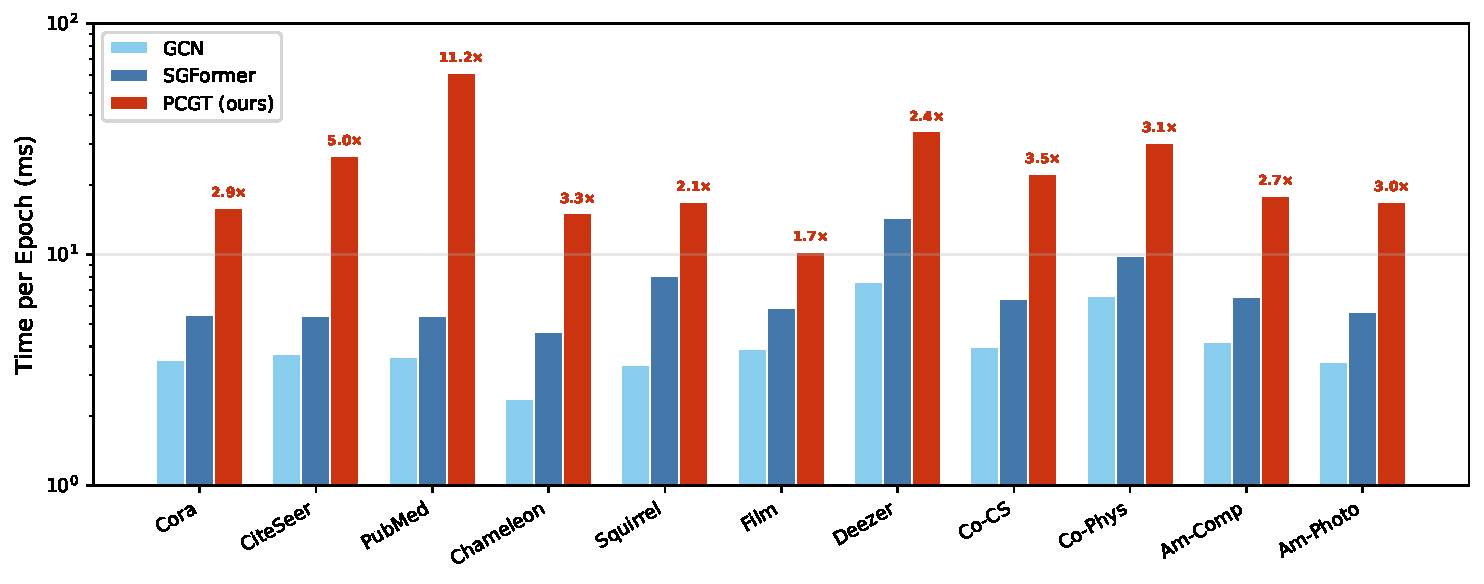
\includegraphics[width=\columnwidth]{figures/runtime_comparison.pdf}
\caption{Per-epoch training time (ms, log scale) on H100. Numbers above PCGT bars show the PCGT/SGFormer overhead ratio. The overhead is moderate and predictable, scaling with $K$ and $N$.}
\label{fig:runtime}
\end{figure}

\section{Sensitivity to Number of Seeds $M$}
\label{app:m_ablation}

Table~\ref{tab:m_ablation} varies the number of learned seeds per partition $M \in \{2, 4, 8\}$ while keeping all other hyperparameters fixed. Performance is stable: the maximum spread is 0.26 points on Cora, 0.94 on Chameleon, and 1.25 on Squirrel---all within one standard deviation. We use $M=4$ throughout.

\begin{table}[t]
\centering
\small
\begin{tabular}{c|ccc}
\toprule
$M$ & \textbf{Cora} & \textbf{Cham.} & \textbf{Sqrl.} \\
\midrule
2 & 84.46{\scriptsize$\pm$0.59} & 47.53{\scriptsize$\pm$2.53} & 46.52{\scriptsize$\pm$1.87} \\
4 & 84.52{\scriptsize$\pm$0.48} & 48.18{\scriptsize$\pm$2.94} & 47.01{\scriptsize$\pm$0.93} \\
8 & 84.26{\scriptsize$\pm$0.84} & 48.47{\scriptsize$\pm$3.04} & 45.76{\scriptsize$\pm$1.11} \\
\bottomrule
\end{tabular}
\caption{Effect of number of seeds $M$ per partition (5 runs each). Differences are within noise; $M=4$ is used throughout.}
\label{tab:m_ablation}
\end{table}

\section{Convergence Behavior}
\label{app:convergence}

Figure~\ref{fig:convergence} shows validation accuracy curves (mean $\pm$ std over 3 seeds) on three datasets spanning homophilic (Cora, PubMed) and heterophilic (Chameleon) regimes. The purpose is to compare \emph{convergence speed}, not final accuracy (which is reported in Table~\ref{tab:main} over 10 runs). Both methods reach plateau validation within similar epoch ranges and trigger early stopping at similar points, confirming that the per-epoch overhead in Table~\ref{tab:runtime} directly translates to total training overhead with no convergence penalty.

\begin{figure}[t]
\centering
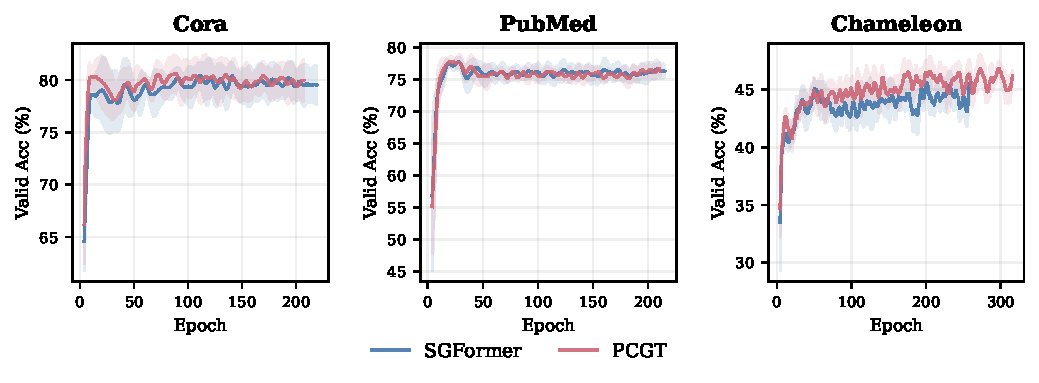
\includegraphics[width=\columnwidth]{figures/convergence.pdf}
\caption{Validation accuracy vs.\ epoch (mean $\pm$ std, 3 seeds) on Cora, PubMed, and Chameleon. Both methods converge at similar speeds. The figure illustrates convergence behavior; final accuracy comparisons use 10-run means (Table~\ref{tab:main}).}
\label{fig:convergence}
\end{figure}

\section{Statistical Significance}
\label{app:significance}

For the four additional datasets (Table~\ref{tab:new_datasets}) where we run both PCGT and SGFormer under identical code, splits, and 10 random seeds, Table~\ref{tab:pvalues} reports Welch's $t$-test $p$-values.  Coauthor-Physics shows a statistically significant improvement ($p = 0.004$), Amazon-Computers is marginally significant ($p = 0.051$), and the remaining two datasets show gains that are within noise.  For the seven Table~\ref{tab:main} datasets, SGFormer baselines are taken from the published numbers of \citet{wu2023sgformer} and per-run data is unavailable, so $t$-tests cannot be computed.

\begin{table}[t]
\centering
\small
\begin{tabular}{l|cc|cc}
\toprule
\textbf{Dataset} & \textbf{PCGT} & \textbf{SGFormer} & $\Delta$ & $p$ \\
\midrule
Co-CS        & 95.06{\scriptsize$\pm$0.32} & 94.94{\scriptsize$\pm$0.46} & +0.12 & 0.240 \\
Co-Physics   & 96.83{\scriptsize$\pm$0.16} & 96.62{\scriptsize$\pm$0.14} & +0.20 & 0.004** \\
Am-Computers & 88.80{\scriptsize$\pm$0.64} & 87.50{\scriptsize$\pm$1.88} & +1.30 & 0.051 \\
Am-Photo     & 95.27{\scriptsize$\pm$0.38} & 95.20{\scriptsize$\pm$1.12} & +0.07 & 0.822 \\
\bottomrule
\end{tabular}
\caption{Welch's $t$-test ($n=10$ runs). $**$: $p < 0.01$.  On homophilic datasets where both methods already perform well, differences are small.  PCGT's largest gains are on heterophilic benchmarks (Table~\ref{tab:main}), where published baselines preclude per-run tests.}
\label{tab:pvalues}
\end{table}

\section{Learned Self-Connection Weight $\beta$}
\label{app:beta}
\label{app:beta_prop}

\begin{proposition}[Sign of optimal $\beta$]
\label{prop:beta}
Let $\mathcal{L}(\beta) = \frac{1}{N} \sum_{i=1}^{N} \ell\bigl(\mathbf{h}_{\text{context},i} + \beta \, \mathbf{V}_i,\; y_i\bigr)$ where $\ell$ is a per-node loss.  If $\mathcal{L}$ is locally convex in $\beta$ near its minimizer $\beta^*$, then
\[
\beta^* < 0 \iff \left.\frac{\partial \mathcal{L}}{\partial \beta}\right|_{\beta=0} < 0 \text{ is false, i.e., } \left.\frac{\partial \mathcal{L}}{\partial \beta}\right|_{\beta=0} > 0.
\]
Equivalently, $\beta^* < 0$ whenever the aggregate gradient $\frac{1}{N}\sum_i \frac{\partial \ell}{\partial \mathbf{h}_i}\Big|_{\beta=0} \!\cdot\, \mathbf{V}_i > 0$, meaning that adding self-features (increasing $\beta$ from 0) increases the loss.
\end{proposition}

\begin{proof}
By the chain rule,
\[
\frac{\partial \mathcal{L}}{\partial \beta} = \frac{1}{N} \sum_{i=1}^{N} \frac{\partial \ell}{\partial \mathbf{h}_i} \cdot \mathbf{V}_i,
\]
where $\mathbf{h}_i = \mathbf{h}_{\text{context},i} + \beta\,\mathbf{V}_i$.  Since $\mathcal{L}$ is locally convex in $\beta$, the function $\beta \mapsto \mathcal{L}(\beta)$ has a unique local minimum $\beta^*$ satisfying $\mathcal{L}'(\beta^*) = 0$.  Convexity implies $\mathcal{L}'$ is non-decreasing, so $\mathcal{L}'(0) > 0$ forces $\beta^* < 0$ (the zero-crossing must be to the left of 0).  Conversely, $\mathcal{L}'(0) < 0$ gives $\beta^* > 0$.
\end{proof}

Table~\ref{tab:beta_values} reports the learned $\beta$ values across all 11 medium-scale datasets (ogbn-arxiv excluded because the large-scale codebase does not log $\beta$).  These values supplement the bar chart in Figure~\ref{fig:beta}.  The two negative-$\beta$ datasets (Film, Deezer) have either noisy, low-dimensional features (Film: 932 dims, actor co-occurrence) or near-random edge labels (Deezer: $h \approx 0.53$), where suppressing self-features improves classification.  The highest $\beta$ values occur on Chameleon and Squirrel, whose high-dimensional Wikipedia features (2325 and 2089 dims) make self-identity highly informative even under low homophily.

\begin{table}[t]
\centering
\small
\begin{tabular}{l|rcc}
\toprule
\textbf{Dataset} & $\beta$ & $h$ & \textbf{Feats} \\
\midrule
Co-Physics   & $+2.09$ & 0.93 & 8,415 \\
Am-Photo     & $+1.75$ & 0.83 & 745 \\
Co-CS        & $+2.08$ & 0.81 & 6,805 \\
Cora         & $+1.19$ & 0.81 & 1,433 \\
PubMed       & $+0.31$ & 0.80 & 500 \\
Am-Computers & $+2.12$ & 0.78 & 767 \\
CiteSeer     & $+2.38$ & 0.74 & 3,703 \\
\midrule
Deezer       & $-0.57$ & 0.53 & 31,241 \\
Chameleon    & $+3.08$ & 0.24 & 2,325 \\
Film         & $-0.99$ & 0.22 & 932 \\
Squirrel     & $+3.53$ & 0.21 & 2,089 \\
\bottomrule
\end{tabular}
\caption{Learned self-connection weight $\beta$ across all medium-scale datasets, sorted by edge homophily $h$.  Positive $\beta$ amplifies the node's own features; negative $\beta$ suppresses them.  Pearson correlation between $\beta$ and $h$: $r = 0.006$, $p = 0.99$.}
\label{tab:beta_values}
\end{table}


\end{document}
